%%%%%%%%%%%%%%%%%%%%%%%%%
% Set up to be stand alone document
% All declerations in the header to be removed when added into thesis
%%%%%%%%%%%%%%%%%%%%%%%%%
% \documentclass[12pt]{article}

% \usepackage{booktabs} % booktabs provides professional formatting commands for tables
% \usepackage{amsmath} % amsmath provides extra maths symbols
% \usepackage{textcomp} % textcomp provides extra text symbols (like a degrees celsius symbol)
% \usepackage{../customisations}
% \usepackage{natbib}

% \title{$J$-band Sythentic Spectral Fitting}
% \date{\today}

% \begin{document}
% \maketitle
%%%%%%%%%%%%%%%%%%%%%%%%%
% To be included when added into thesis
\chapter{J-band Spectral Analysis}\label{ch:janal}

\section{Opening Remarks} % (fold)
\label{sec:opening}

In this chapter I describe in detail the process by which I implement an analysis
routine to fit synthetic spectra to observed data with the aim of estimating stellar parameters.
This analysis builds on existing methods while providing a fresh approach to various aspects of the routine.
I have developed this implementation in the public domain and the source code for this project is made publicly available
via an online repository.\footnotemark

\footnotetext{Source code available from: https://github.com/lrpatrick/rsg-janal
although the interested reader should be aware that these routines are, at the time of writing, in development mode
in the sense that they are highly specialised to one machine and (particularly) one set of model grids}

In this chapter I first outline the principles of model atmospheres in Section~\ref{sec:model_atmospheres}, where I discuss the physics which is included in these models as well as some of their strengths and limitations.
I then focus the discussion on the grid of synthetic stellar spectra which forms the base of this analysis routine in Section~\ref{sec:model_grid}.
In Section~\ref{sec:continuum_fitting} I detail the procedure of matching the continuum level of the observations with that of the models,
which leads on to Section~\ref{sec:best_fit_parameters}, where the method by which the best fit parameters are selected is described.

Having described the analysis routine thoroughly I then test this routine and compare the results of this method to different implementations in the literature in Section~\ref{sec:calibration}.
Finally, I conclude the chapter in Section~\ref{sec:conclusions}.

% section opening (end)
\section{Introduction to Stellar Model Atmospheres} % (fold)
\label{sec:model_atmospheres}

A stellar atmosphere is defined as the outer layers within a star which emit radiation.
Therefore, by definition, the photons which we observe from a star have originated in the atmosphere.
Photons which have originated from deeper layers within the star have been absorbed and re-emitted by particles within the stellar atmosphere.
Stellar atmospheres are therefore vitally important in observational studies of stars, even though the fraction of the total mass of the star contained within the atmosphere is tiny ($\sim$~10$^{-10}$).
A nice analogy for visualising this layer and its thickness comes from the preface of~\cite{1989isa2.book.....B}, where these authors compared the skin of an apple to a hypothetical star which has been shrunk to the same scale and note that the skin of the apple is far thicker than the stellar atmosphere.


Even though stellar atmospheres contain a tiny fraction of the total stellar mass, these layers can have an enormous impact on the evolution of a star via stellar winds.
For example, in evolved massive stars, winds arising from the atmosphere can strip off the outer layers of the star to leave an exposed hydrogen and helium dominated core or push the star in a completed different evolutionary direction to become a RSG (see Chapter~\ref{ch:intro}).
In addition to having an impact on the evolution of the star, winds also help distribute material throughout their host galaxy and feed subsequent generations of star formation~\citep[e.g.][]{2011MNRAS.417..950H,2012MNRAS.421.3522H} thereby not only affecting the evolution of the star in which the wind is produced, but by acting as part of a larger stellar population, affect the evolution of their host galaxy.

By modelling stellar atmospheres, one can estimate fundamental stellar parameters by a comparison with observations.
The background theory and underlying physical assumptions of these models is the subject of the current section.
This is important to detail as without this background it is impossible to assess the effectiveness of the models and their limitations.

Two of the most fundamental equations which govern the properties of stellar atmospheres are,

\begin{equation}
    g = \frac{GM}{R^2},\label{eq:grav}
\end{equation}

\noindent and,

\begin{equation}
    \Teff = \frac{F}{\sigma_{SB}} = \left(\frac{L}{4\pi \sigma_{SB}R^2}\right)^\frac{1}{4},\label{eq:Teff}
\end{equation}

\noindent where $g$ is the acceleration due to gravity, $M$ is the total mass of the star of radius $R$, \Teff is the effective temperature of the star, $F$ is the total flux per unit area, $L$ is the total luminosity of the star, $\sigma_{SB}$ is the Stefan-Boltzmann constant and $G$ is Newton's gravitational constant.

These equations define some fundamental observational properties of the model stellar atmospheres.
Equation~\ref{eq:grav} is defined by the density stratification of the model and equation~\ref{eq:Teff} is defined through the total flux emitted from the model.

In the following sections I detail three of the principle assumptions which are used to create a ``classical'' one dimensional stellar model atmosphere.
These assumptions underpin some of the most widely used model atmospheres.


\subsection{Hydrostatic Equilibrium} % (fold)
\label{sub:hydrostatic_equilibrium}

Any model of a star consists of a balance between gravity and pressure in a gaseous material (or plasma considering the typical temperatures and densities within a star).
If a model is assumed to be static (i.e. not varying with time) the equation of hydrostatic equilibrium can be derived by considering the balance between forces acting upon a small element of stellar material,

\begin{equation}
    \frac{dP(r)}{dr} = -\frac{\rho GM(r)}{r^2},\label{eq:hydro}
\end{equation}

\noindent where $P$ is the total pressure exerted within a radius $r$, $M$ is the total mass within a radius $r$, $\rho$ is the matter density~\citep[see Chapter 9 of ][for a simple derivation of this equation]{1989isa2.book.....B}.
As stated above, the mass contained within the atmosphere of a star is a negligible fraction of the total mass, therefore $M(r) = M_{tot}$ when considering this equation in the outer layers of the star.

The force exerted by pressure acting on an element of stellar material ($dP/dr$) can be considered as the sum of the forces acting upon it from gas pressure ($P_{g}$), radiation pressure ($P_{rad}$) and turbulent pressure ($P_{turb}$),

\begin{equation}
    \frac{dP_{tot}}{dr} = \frac{dP_{g}}{dr} + \frac{dP_{rad}}{dr} + \frac{dP_{turb}}{dr}.\label{eq:pressure}
\end{equation}

Equation~\ref{eq:pressure} illustrates that even though we have assumed the model is static, small scale turbulent motions must still be taken into account to accurately model stellar atmospheres.


% subsection hydrostatic_equilibrium (end)

\subsection{Mixing Length Convection} % (fold)
\label{sub:mlt}

Mixing length theory describes how convection is treated within the stellar atmosphere.
Typically, within a star, radiation is the main source of energy transport as the coefficient of diffusion is far smaller for particles (conduction) than for photons (radiation).
Only in degenerate cores does energy transport via conduction become important.

Convection is a very efficient form of energy transport where a macroscopic element of higher temperature rises an average distance into a region of lower temperature where it dissipates the excess energy being carried and mixes.
However, in order for convection to be effective, a driving mechanism must be established.
The atmosphere is unstable to convection if the Schwarzschild criterion is met,

\begin{equation}
    \nabla_{rad} > \nabla_{ad}
\end{equation}

\noindent where $\nabla_{rad} = (d~{\rm ln}\,T/d~{\rm ln}\,P)_{rad}$ is the radiative temperature gradient and $\nabla_{ad}$ is the adiabatic temperature gradient.
The driving mechanism for convection is usually a large temperature gradient within a particularly part of the star.
This can occur at various stages within the lifetime of a star, for example, most main sequence stars have a convective core which is a result of the temperature sensitivity of the CNO cycle which establishes a steep temperature profile.

The theory of convection is very difficult to to treat thoroughly.
The ``simple'' theory of mixing length convection~\cite{1958ZA.....46..108B,1965ApJ...142..841H} is widely used to implement convection within stellar atmospheres which assumes that the shapes and sizes of the elements which transport energy is fixed and that, on average, an element rises a characteristic length ($l_m$) before it dissipates energy.

If the Schwarzschild criterion is satisfied, the total flux ($F$) for a star is given by,

\begin{equation}
    F(r) = F_{conv} + F_{rad} = \sigma T_{eff}^4,\label{eq:flux}
\end{equation}

\noindent where $F_{conv}$ and $F_{rad}$ are the convective and radiative flux respectively.
An expression for the convective flux can be obtained by considering the excess energy dissipated by a rising element moving a distance
($\Delta r = l_m/2$) with an average velocity ($v_{conv}$).
The convective flux can therefore be expressed as,

\begin{equation}
    F_{conv} = \rho C_pv_{conv}\Delta T,
\end{equation}

\noindent where $C_p$ is the specific heat at constant pressure and $\Delta T$ is the temperature difference between the element and surroundings, which can be expressed in terms of the different in temperature gradients.
Here the pressure scale height can be introduced using the assumption of hydrostatic equilibrium $H_p = dr / d{\rm ln} P = p/\rho g$ and an expression for the convective velocity can be estimated by assuming that half the work done by buoyancy is converted into kinetic energy,

\begin{equation}
    \frac{1}{2}\langle w\rangle \approx \frac{1}{2}\rho v_{conv}^2.
\end{equation}

The parameter $\alpha = l_m/H_p$ is introduced which typically takes the value $\alpha$ = 1.5--2.0.
As a side note, in stellar evolutionary models, the value of $\alpha$ used can have a significant effect on the temperature of the models at the end of the RSG phase of evolution.


% subsection mlt (end)

\subsection{Local Thermodynamic Equilibrium} % (fold)
\label{sub:local_thermodynamic_equilibrium}

The assumption of thermodynamic equilibrium is where the temperature and density of a material can be considered constant (i.e. there are no net flows of energy).
Which is equivalent to assuming that the emitting source is a perfect black body.
Local thermodynamic equilibrium (LTE) is an approximation whereby the {\it local} properties of material can be assumed to be in thermodynamic equilibrium.
Stellar atmospheres can be approximated to be in LTE as their densities are sufficiently high and density gradients are sufficiently low that their local properties are closely related to thermal equilibrium.

The three fundamental equations which can be defined assuming LTE are:

\begin{enumerate}
    \item The Boltzmann equation,
    \begin{equation}
        \frac{n_i}{N_I} = \frac{g_i}{U_I}e^{-E_i/kT},\label{eq:boltz}
    \end{equation}
    \item The Saha equation,
    \begin{equation}
        \frac{N_I}{N_{I+1}} = n_e\frac{U_I}{U_{I+1}}\left(\frac{h^2}{2\pi m_ekT}\right)^\frac{3}{2} e^{\chi/kT},
        \label{eq:saha}
    \end{equation}
    \item The Maxwellian distribution of particles,
    \begin{equation}
        f(v)dv = \left(\frac{m}{2\pi kT}\right)^\frac{3}{2} \exp\left(\frac{-mv^2}{2kT}\right)4\pi v^2dv,
        \label{eq:max}
    \end{equation}
\end{enumerate}

\noindent where $n_i$, $g_i$ and $E_i$ are the population, statistical weight and energy of level $i$ respectively,
$N_I$, $U_I$ and $\chi_I$ are the total number density, partition function and ionisation potential of ionisation state $I$ (to which $i$ belongs),
$m$ is the mass of the particle, $v$ is the velocity of the particle, $T$ is the temperature of the particle and $k$ is the Boltzmann constant.
Equation~\ref{eq:boltz} determines the level population of a particular ionisation state for a given atom and in combination with the Saha ionisation equation (equation~\ref{eq:saha}) is used to determine the total level population for a given atom.

% These three equations describe the


% In addition the radiation source function (in the MARCS models -- not always the case) is assumed be be

% \begin{equation}
%     S_\lambda = \frac{\kappa_\lambda}{\kappa_\lambda + \sigma\lambda}B_\lambda(T) + \frac{\sigma_\lambda}{\kappa_\lambda + \sigma\lambda}J_\lambda
% \end{equation}

% More generally, in thermodynamic equilibrium $S_\lambda = B_\lambda$.
% In LTE

% subsection local_thermodynamic_equilibrium (end)

\subsection{Analysis of Assumptions and Summary} % (fold)
\label{sub:assumptions_summary}

The assumptions listed above allow one to obtain to create a ``standard'' stellar model atmosphere.
The assumptions listed above are known to be simplifications of the true picture with a stellar atmosphere.
For example, the assumption of LTE definitely breaks down in the atmospheres of stars as they are observed and, by definition, emit radiation.
However, using the above assumptions one can build a consistent model that, in general, agrees reasonably well with observations.

The treatment of convection is knowingly a large simplification as the shape and size assumed for the convective elements is constant whereas in reality the shapes of these elements could be described as funnel-like.
Full two- and three-dimensional hydrodynamical simulations are required to assess the assumption of mixing length convection which generally show that convective fluxes are smaller than those in more sophisticated prescriptions
\citep{2012sse..book.....K}.

The assumption of LTE typically holds in dense low levels of a star, however, in the atmosphere, where radiation is emitted, this is known to be a poor approximation.
This is particularly true in evolved stars where departures from LTE are expected owing to the low densities and surface gravities of their atmospheres.

Full non-LTE stellar model atmospheres are expensive to produce and are only available for particular sets of stellar parameters~\citep[e.g. {\sc tlusty} for stars with \Teff~$<$~27\,500;][]{2003ApJS..146..417L}
as of yet, there exists no homogeneous grid of model atmospheres which include these effects for cool stars.
As a first step, one can use a homogeneous set of model grids computed in LTE and select particular elements with which to compute non-LTE deviations in a particular wavelength regime.
This is far less time expensive and produces reliable results over a large range of stellar parameters.


% subsection analysis_of_assumptions_and_summary (end)

% section model_atmospheres (end)

\section{Quantitative Analysis of near-IR Spectroscopic Observations} % (fold)
\label{sec:model_grid}

To compare stellar model atmospheres to near-IR spectroscopic observations, synthetic spectra are calculated.
By calculating synthetic spectra from a grid of model atmospheres with a range of physical parameters, one can then compare the models to observations and determine the model, and hence stellar parameters, which best reproduces the data.
There are four model parameters which are considered to affect the appearance of the spectra:
global metallicity ($\log (Z/Z_{\odot})$~=~[Z]), effective temperature (\Teff), surface gravity ($\log\,g$) and microturbulence ($\xi$).
Microturbulence is a non-thermal velocity which is included in quantitative analyses of stellar spectroscopic observations in order to fit the observed line profiles.
For MS stars, empirical microturbulence velocities are thought to be connected with convective overshoot motions in stellar atmospheres~\citep{2009A&A...499..279C} and/or the result of high-order non-radial pulsations~\cite[e.g.][]{2015ApJ...806L..33A}.


The synthetic spectra used in this analysis cover the $J$-band, specifically the $1.16-1.22\mu$m region.
The wavelength range is chosen based on the spectral appearance of the region.
Typically, in the spectra of cool stars, dense molecular absorption features dominate the spectrum which require high-resolution spectroscopy to distinguish individual features and estimate stellar parameters~\citep{Cunha07, Davies09a, Davies09b}.
However, in this small wavelength range the absorption is dominated by well separated elemental absorption features from iron, magnesium, silicon and titanium.
Therefore, the spectral resolution required in order to derive stellar parameters is significantly reduced.
This means that this analysis, unlike others at higher resolution, can be performed with a relatively small amount of telescope time using near-IR multi-object spectrographs like KMOS on the VLT
or the multi-object spectrometer for infra-red exploration (MOSFIRE) on Keck and is therefore feasible for studies of large populations of RSGs in external galaxies.

In addition to this, given the cool temperature of the outer layers of RSGs,
the peak brightness of a typical RSG is $\sim\,1.1\mu$m.
Combining this with the fact that dust attenuation is significantly lower in the near-IR, compared to the optical regime, RSGs are ideal candidates to be studied at large distances.

At near-IR wavelengths, the effects of absorption and emission from the Earth's atmosphere is a considerable complication.
Although an absorption line may be strong and well separated from other stellar features, it may be contaminated by features arising from the Earth's atmosphere.
If a stellar feature is contaminated with strong absorption or emission arising from the Earth's atmosphere (telluric or sky line respectively), the correction required to divide or subtract the non-stellar feature may well leave behind residuals which perturb the line strength or shape.
For example, in Figure~\ref{fig:tell3pan} there are two strong iron lines around 1.16\,$\mu$m in the synthetic spectrum (top panel) which are well separated and would be suitable for the estimation of stellar parameters.
However, when telluric contamination is taken into account, we can see that the size of the telluric absorption around these lines is comparable to the strength of the lines (middle panel).
By correcting for the effects of the Earth's atmosphere we introduce a significant uncertainty in the strength and shape of these lines.
Therefore, these lines are unsuitable to be used to measure stellar parameters.
Equally, Figure~\ref{fig:skysub} in Chapter~\ref{ch:kmos} demonstrates the sky emission lines can also leave behind significant residuals that can perturb stellar features.
The diagnostic features therefore must be chosen carefully by examining not only the model RSG spectra, but by also taking into account potential reduction residuals arising from the Earth's atmosphere.
However, if one observes above the Earth's atmosphere, these lines - and many others - could be used to estimate stellar parameters.

\begin{figure}
 \centering
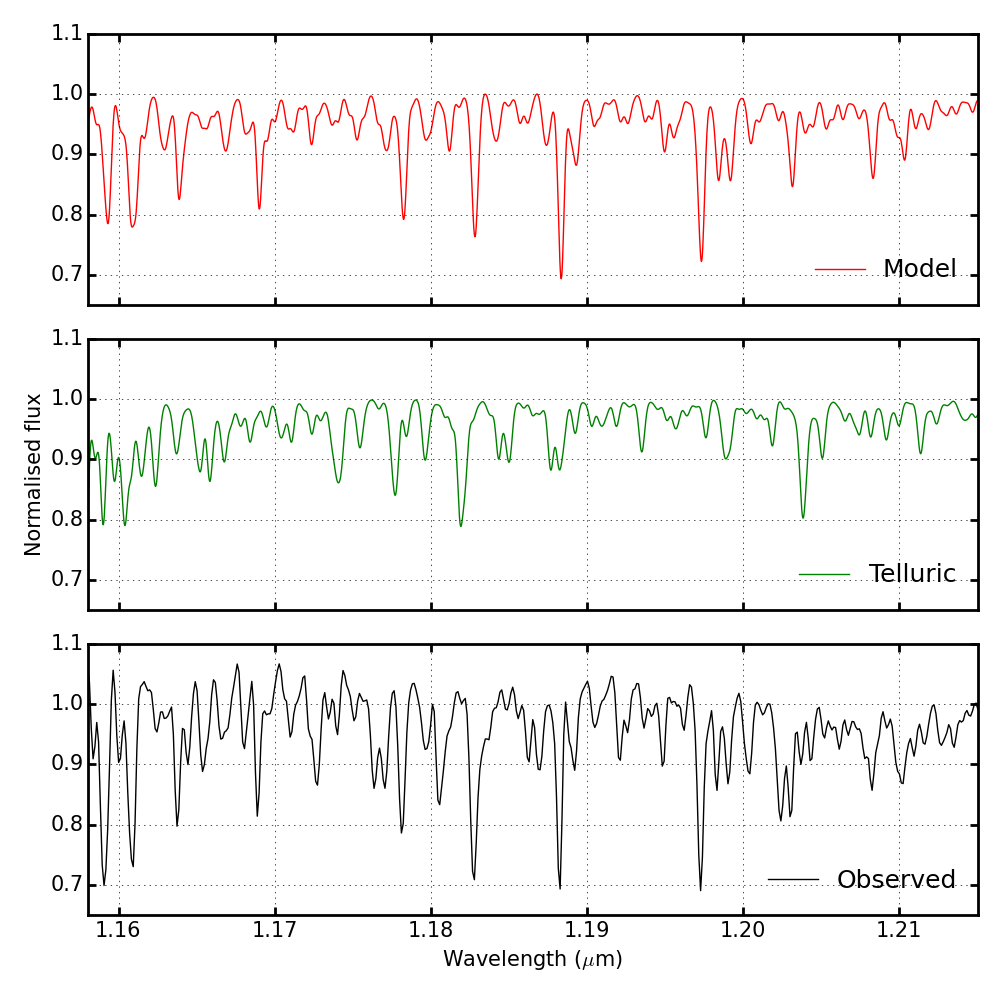
\includegraphics[width=\textwidth]{JAnal/tell-correction}
\caption{
Three panels showing the effect of telluric absorption on spectral lines.
The top panel shows a synthetic RSG spectrum within the wavelength of interest.
The middle panel shows a spectrum of the Earth's atmosphere and
the bottom panel shows an observed KMOS spectrum without telluric correction which is a combination of the top two panels and a noise spectrum.
To illustrate that the lines used in the analysis must come from regions where there is little telluric contamination, I draw the readers attention to the two iron lines at 1.16\,$\mu$m.
Even though these lines are well separated in the model spectra, telluric contamination renders these lines unsuitable for the estimation of  stellar parameters and one can see that the shape of these lines is altered by strong telluric contamination.
\label{fig:tell3pan}
         }
\end{figure}

% Previous studies which have used this wavelength regime to estimate stellar parameters for RSGs consist of that of
% \cite{2010MNRAS.407.1203D} and~\cite{2014PhDT.........G}.
% This implemenation includes aspects of both of these previous implementations and could be described as a hybrid of the two.
% Eventually this analysis routine will be made publicly available will should encourage the community to engage with these routines.

The synthetic spectra used in this analysis are calculated from model atmospheres computed from the MARCS model atmospheres project
\citep{1975A&A....42..407G,2008A&A...486..951G}.
These model atmospheres are ``standard'' type models computed in one-dimension (i.e. spherically symmetric)
where hydrostatic equilibrium, mixing-length theory of convection and LTE are assumed.
The MARCS models are particularly general and widely applicable to many different types of stars and as such are well used and tested.
However, for the atmospheres of RSGs the assumptions which go into these models (LTE in particular) are known to break down
\citep{2002AN....323..213F,2010ASPC..425..124P}.
Therefore, in order to accurately analyse the spectra of RSGs additional corrections must be applied~\citep{2012ApJ...751..156B}.

The MARCS model atmospheres used for this analysis are computed with a mass of 15\,M$_{\odot}$.
The typical mass range of a RSG is 8~$\leq$~M/M$_{\odot}$~$\leq$~40, however,
using this mass is applicable owing to the fact that altering the mass of these models affects only the extension
(or geometrical thickness) of the atmosphere which does not change substantially for red giants or supergiants
\citep[see][]{2010MNRAS.407.1203D}.

To improve the accuracy of the model atmospheres,
non-LTE calculations have been performed for all elements which give rise to the diagnostic features within the wavelength range studied
\citep{2012ApJ...751..156B,2013ApJ...764..115B,2015ApJ...804..113B}.
The line formation calculations of all known transitions of important atoms and molecules are computed in non-LTE using the {\sc detail} code~\citep{1981PhDT.......113G}.
{\sc detail} is a well tested and widely used code which is used to solve statistical equilibrium equations to obtain non-LTE level populations.
Using these level populations, line profiles and synthetic spectra -- with non-LTE corrections for the key diagnostic lines -- are calculated using an updated version of the {\sc SIU} code~\citep{1999PhDT.........3R,2012ApJ...751..156B} which employs the same input physics as {\sc detail}.
By calculating synthetic spectra from a grid of stellar models one can then evaluate which combination of model stellar parameters best represents the observed dataset.

The parameters of the resulting grid of synthetic spectra are detailed in
Table~\ref{tb:grid} where the spectral resolving power is $R$~=~10\,000,
which is significantly higher than the typical resolving power of the observed spectra
(i.e. $R \sim 3000$).
The sensitivity of each diagnostic line for a given free parameter is illustrated in Figures~\ref{fig:mod-z} through~\ref{fig:mod-micro} where one parameter is varied and the remaining are fixed.

\begin{table}
\caption{Model grid parameter space\label{tb:grid}}
\scriptsize
\begin{center}
\begin{tabular}{lccc}
 \hline
 \hline
Parameter & Abbreviation & Range & Increment \\
 \hline
Global metallicity & $[Z]$ & +1.0~--~$-$1.0 & 0.1\,dex \\
Effective Temperature & \Teff & 3400~--~4400 & 100\,$K$ \\
Surface gravity & $\log g$ & +1.0~--~$-$1.0 & 0.25\,dex \\
Microturbulence & $\xi$ & 1.0~--~5.0 & 0.2\,$km\,s^{-1}$ \\
 \hline
\end{tabular}
\end{center}
\end{table}




\begin{figure}
 \centering
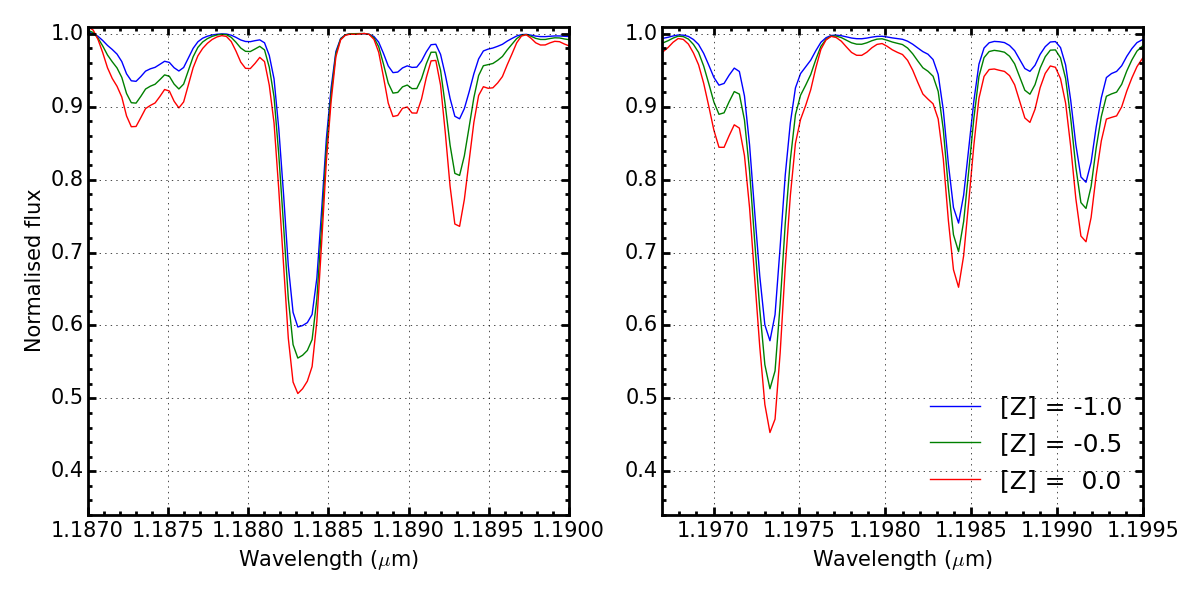
\includegraphics[width=\textwidth]{JAnal/varyZv2}
\caption{
Three example models where only the metallicity is varied, the remaining stellar parameters are fixed at \Teff = 3900\,K, $\log g$ = 0.0 and $\xi$~=~3.0\kms.
Five diagnostic lines are shown in the two panels.
Left: Fe\,I $\lambda$1.188285 and Ti\,I $\lambda$ 1.189289.
Right: Fe\,I $\lambda$1.197305 and Si\,I $\lambda\lambda$ 1.198419, 1.199157.\label{fig:mod-z}
         }
\end{figure}
\begin{figure}
 \centering
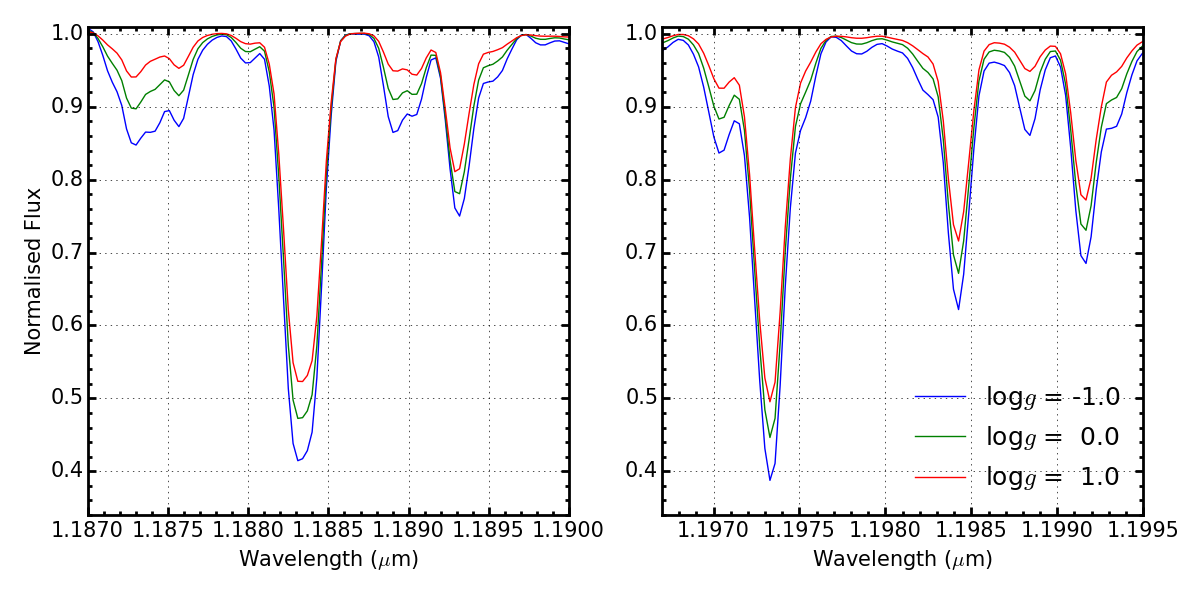
\includegraphics[width=\textwidth]{JAnal/varygv2}
\caption{
As in Figure~\ref{fig:mod-z} where surface gravity is varied and the remaining parameters are fixed at [Z] = $-$0.5, \Teff = 3900\,K and $\xi$~=~3.0\kms.\label{fig:mod-g}
         }
\end{figure}


From an analysis of Figures~\ref{fig:mod-z} and~\ref{fig:mod-g} it can be seen that the effect of increasing the metallicity of the models is similar to that of decreasing the surface gravity.
It is therefore expected that a degeneracy exists between metallicity and surface gravity.
This degeneracy is explored further in Section~\ref{sec:best_fit_parameters}.

The effect of varying the temperature of the models changes the relative strengths of the lines of different spectral species.
For example, see the left panel in Figure~\ref{fig:mod-t} where the ratio of the iron
($\lambda\,1.188285$) to titanium ($\lambda\,1.189289$) lines is strongly affected by varying the temperature of the models.
Also note that each species does not respond linearly to temperature.
This can be seen by a comparison between the strength of the iron line
($\lambda\,1.197305$) in the right hand panel of figure~\ref{fig:mod-t} to that of the silicon lines
($\lambda\lambda\,1.198419, 1.199157$) in the same panel.
This is clearly distinguishable from all the effects of all other parameters.


Increasing the microturbulence has the effect of increasing the equivalent widths
of the strongest lines preferentially as well as affecting the relative strengths of the lines arising from the same spectral species.
Therefore, strong features arising from the same element will be most sensitive to this
parameter.
This is illustrated by a comparison between the two strong iron lines
($\lambda\lambda\,1.188285, 1.197305$) in the left and
right panel of Figure~\ref{fig:mod-micro}.
Where the iron line in the left panel is strongest at $\xi~=~1.0$,
whereas at $\xi~=~5.0$, the iron line in the right panel is the stronger of the two.
In addition, the relative strengths of the two silicon lines
($\lambda\lambda\,1.198419, 1.199157$) in the right hand panel are not strongly affected, which illustrates that microturbulence preferentially affects the strongest spectral features.

\begin{figure}
 \centering
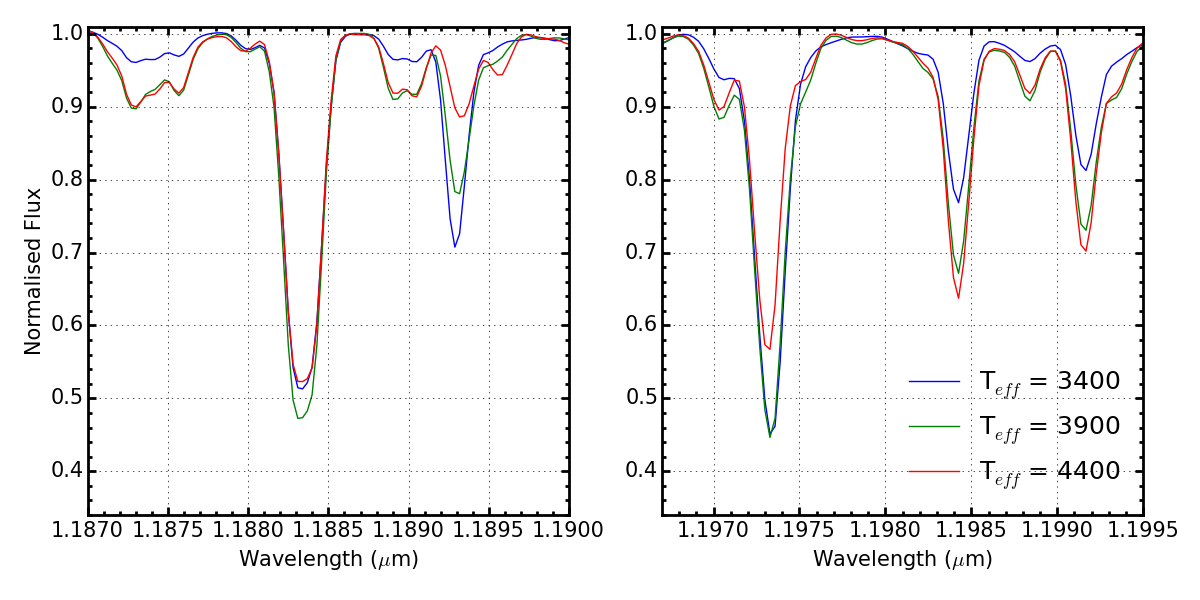
\includegraphics[width=\textwidth]{JAnal/varyTv2}
\caption{
As in Figure~\ref{fig:mod-z} where effective temperature is varied and the remaining parameters are fixed at [Z] = $-$0.5, $\log g$ = 0.0 and $\xi$~=~3.0\kms.\label{fig:mod-t}
         }
\end{figure}
\begin{figure}
 \centering
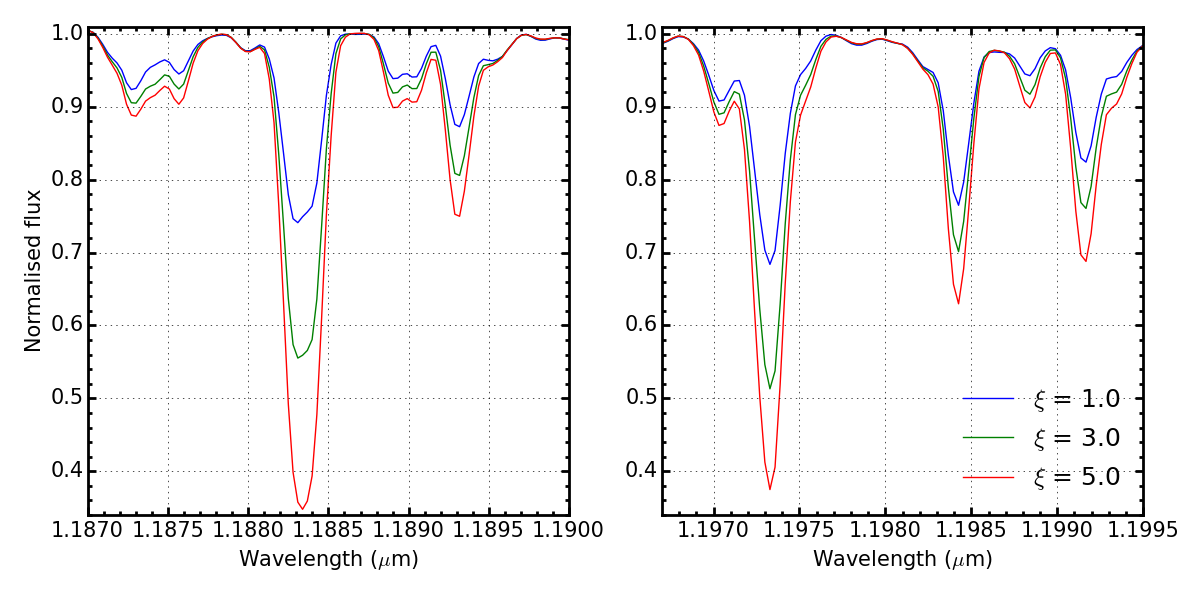
\includegraphics[width=\textwidth]{JAnal/varymicrov2}
\caption{
As in Figure~\ref{fig:mod-z} where microturbulence is varied and the remaining parameters are fixed at [Z] = $-$0.5, \Teff = 3900\,K and $\log g$ = 0.0.\label{fig:mod-micro}
         }
\end{figure}

The current model grid is sufficient to explore the parameters for a typical RSG in the Local Universe.
However, when using this technique at larger distances,
many different metallicity environments are encountered e.g. the low metallicity environment of I\,Zw\,18 with $Z=(1/32)Z_{\odot}$~\citep{1998ApJ...508..248V}.
In order to study these extremely low-metallicity systems,
the metallicity parameter space would need to be extended.
The $\alpha$-to-iron ratio of these stars is taken to be that of the solar value and is not yet left as a free parameter in the models.
This is applicable as young stars are known to have solar-like $\alpha$-to-iron ratios in different metallicity galaxies
~\citep[see tables 3 and 4 in][and references therein]{2015ApJ...806...21D}.

% section model_grid (end)
\section{Continuum Fitting} % (fold)
\label{sec:continuum_fitting}

Accurately matching the continuum levels in the observed
spectrum provides a base with which to anchor the comparison of the diagnostic lines of the models.
An incorrectly placed continuum level would bias the analysis and result in the
strength of the diagnostic lines being over- or under-estimated producing inaccurate stellar parameters.

% The continuum fitting procedure is important because determining the base of the
% diagnostic lines defines their overall strength which is used to distinguish
% between models.
There are many factors that affect the level of the continuum and continuum placement,
including the resolution of the observations as well as the stellar parameters themselves.
Therefore it is vital that when attempting to derive stellar parameters,
in crowded spectral regions such as this, the continuum placement is performed
consistently and accurately.
Intrinsically, when studying RSGs at medium resolution --- owing  to their cool atmospheres ---
there are many instances of blended spectral features.
At this resolution the density of blended spectral features creates a pseudo-continuum which, in practice,
is never at the true continuum level.
Figure~\ref{fig:mod-res} illustrates the varying continuum levels for models where the resolution is varied and
Figures~\ref{fig:mod-z}--\ref{fig:mod-micro} show that varying each of the stellar parameters affect the continuum in a subtly different manner.

\begin{figure}
 \centering
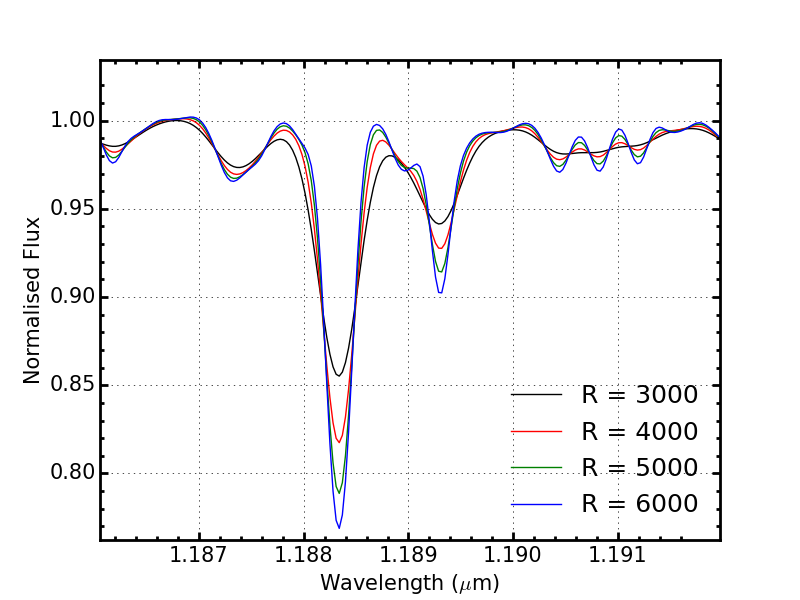
\includegraphics[width=0.65\textwidth]{JAnal/Resolution}
\caption{
One model degraded to four different resolution values.
This figure demonstrates the how the continuum level changes depending upon
the resolution of the spectrum.
We see at around 1.191\,$\mu$m at $R$~=~3000 the continuum level is perturbed by blended lines.\label{fig:mod-res}
         }
\end{figure}

% \begin{figure}
%  \centering
% 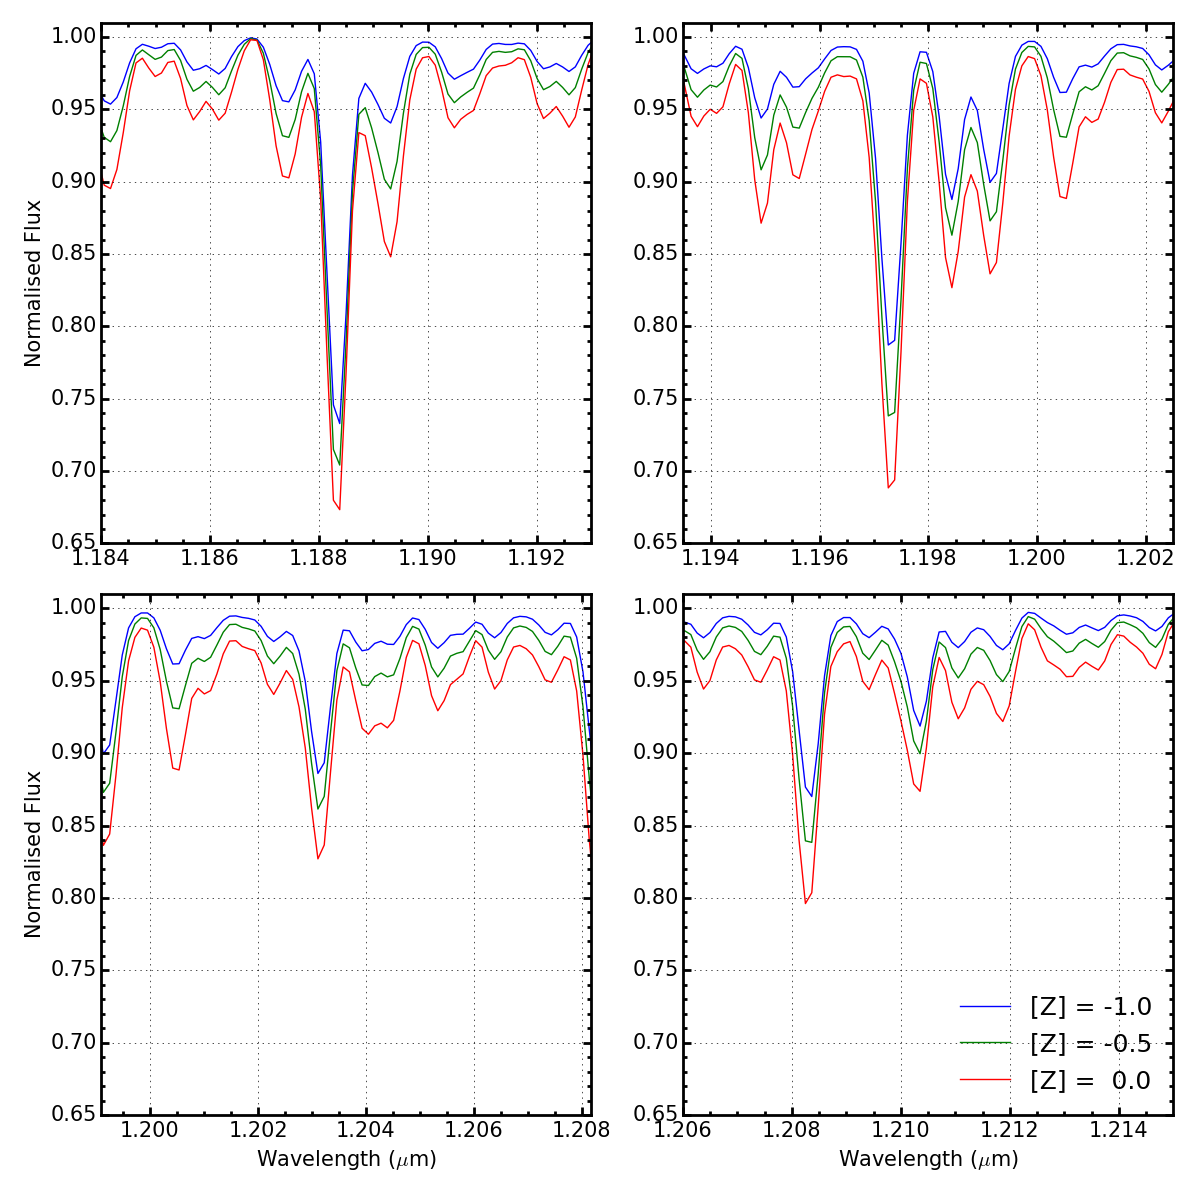
\includegraphics[width=0.65\textwidth]{JAnal/varyZ}
% \caption{
% Three models where only the metallicitiy is varied.
% Each panel shows one or more diagnostic line.
% Metallicity of the model intrinsically affects the continuum level of the spectrum,
% such that at higher metallicities, there is greater departure from the true continuum level, which in the case of the models is 1.00.\label{fig:mod-zcont}
%          }
% \end{figure}


Given that it is impossible to know the true continuum level from any given observation,
the scaling applied must be consistent between the models and observations.
Scaling is required not only to match the levels of the continuum placement, but also to match the line strengths between the models and observations.
Providing the treatment of the models and observations are consistent, the fact that the true continuum is never attained is not significant
\citep{2014ApJ...788...58G}.
For the process of continuum matching to work effectively,
the observed and model spectra should be at the same resolution,
have a consistent wavelength calibration and have identical spectral sampling.

In order to account for differences in the spectral sampling of the observed and model spectra,
each model spectrum is resampled onto the wavelength scale of the observations by means of a spline interpolation routine.
The model spectrum is then degraded to the resolution of the observations by a
convolution with a Gaussian filter where the width of the Gaussian is defined by the observed resolution ($FWHM~=~\sqrt{(\lambda/R)^{2} -(\lambda/R_{mod})^{2}}$ where $R$ is the spectral resolving power of the observed spectrum).
The spectral resolving power of the KMOS observations is estimated using the KMOS/esorex pipeline from arc lamp exposures at the appropriate rotator angle for the observations.
This is measured for each spectrograph and is assumed to be constant (to within $\pm$\,100) across individual IFU's as well as across the detector.

To ensure the spectra are on the same wavelength scale, the observed spectrum is cross-correlated with the model spectrum;
a shift is then applied to the model spectrum in order to minimise the cross-correlation matrix.
This procedure is repeated until the shift between the observed and model spectra is less than 0.1\,pixel.
Over this small wavelength range, one would not expect significant variations in the spectral resolution of the observations to perturb the cross-correlation.

Once the spectra have been correctly matched they are now suitable to be compared over the wavelength range 1.165--1.215$\mu$m.
To estimate the amount of scaling required first I define the continuum width ($cw$) as:

\begin{equation}
    cw~=~\frac{\lambda}{R}, %\times S,
\end{equation}
\noindent where $R$ is the resolution of the spectrum and
$\lambda$ is the wavelength at which the width is taken
(in principle this wavelength varies across the spectrum, however, given our spectral window is sufficiently small, I assume $\lambda$~=~1.20\,$\mu$m).
% and $S$ is a scale factor which takes the range $0.5 < S < 1.0$.
The continuum width is essentially the resolution element of the spectrum at a wavelength of
$\lambda$~=~1.20\,$\mu$m.

The model spectrum is divided into wavelength slices each of width $cw\mu$m and the maximum of each slice is taken.
Using this array of maxima any major feature is systematically removed by rejecting data points more than 3\,$\sigma$ from the mean of the distribution.
Figure~\ref{fig:cw} illustrates the width of these slices and how this technique removes prominent spectral features.
In this figure blue points represent the boundaries between the slices of width $cw\,\mu$m and the maximum of each slice is shown in red.


\begin{figure}
 \centering
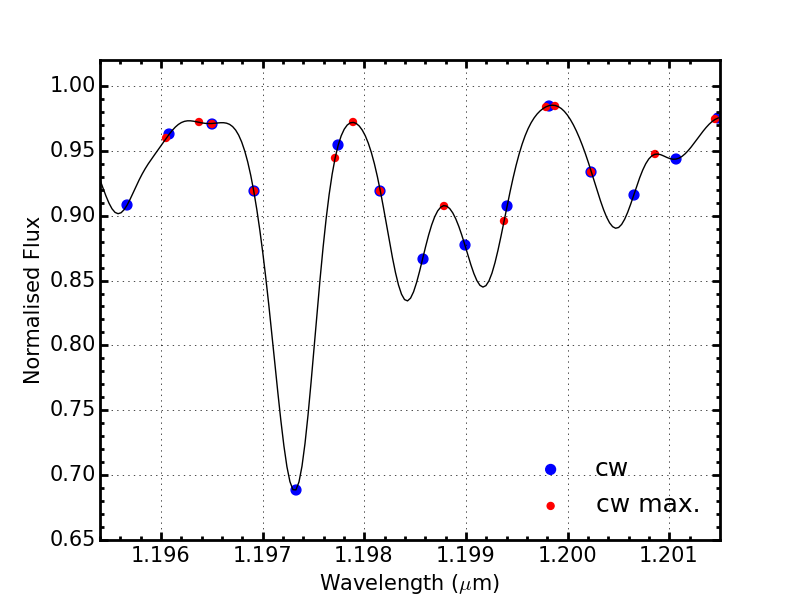
\includegraphics[width=0.65\textwidth]{JAnal/cw}
\caption[Illustration of continuum width slices and maxima]{
Illustration of the continuum width ($cw$) and slicing the model spectrum into regions of $cw\mu$m is able to remove structure in order to fit the continuum.
The solid black line shows an example of a model spectrum degraded to a resolution of 3000,
blue points show the boundaries between the slices and red points show the maximum of each slice.\label{fig:cw}
         }
\end{figure}


\begin{figure}
 \centering
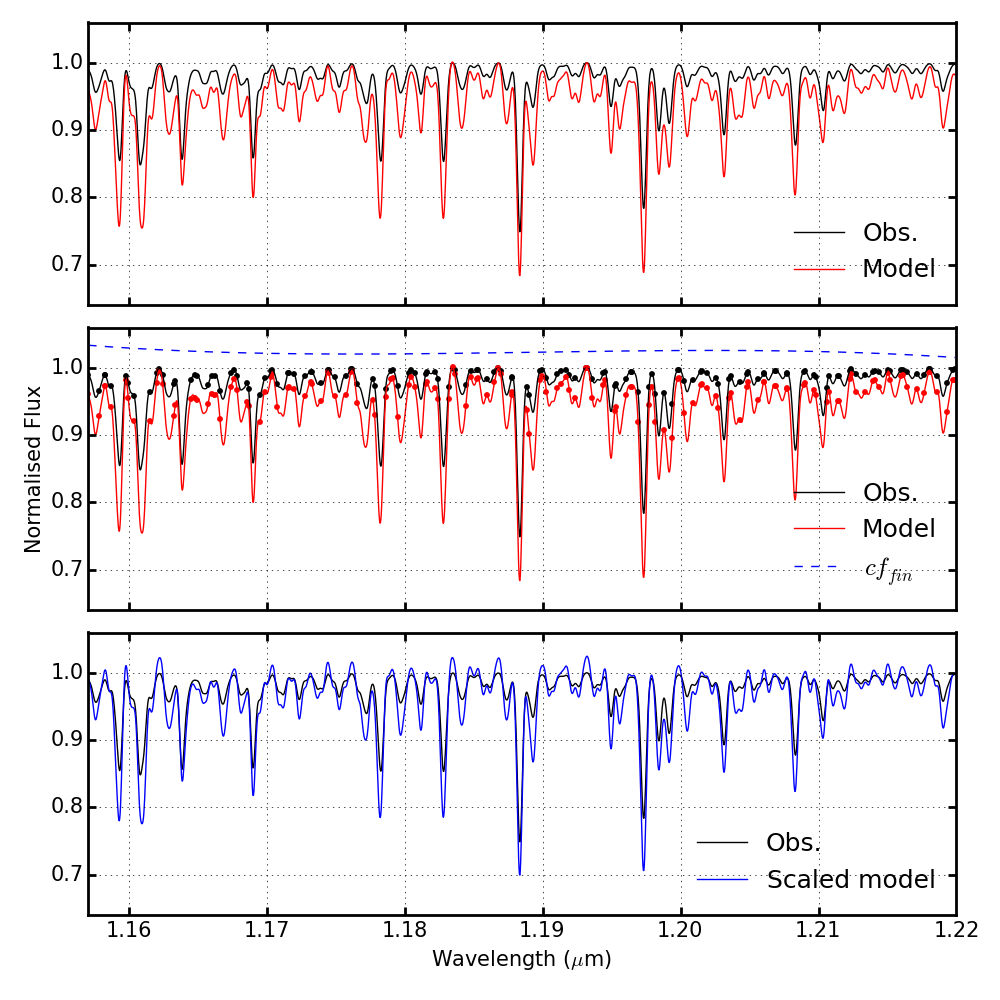
\includegraphics[width=\textwidth]{JAnal/cw-3panels}
\caption[Continuum fitting procedure]{
Three panels showing an example of how the continuum fitting works using a model spectrum as an example observed spectrum (black solid line) and a separate model spectrum to match the level of the continuum (red solid line).
The top panel shows the observed spectrum (black solid line) compared with the unscaled model spectrum (red solid line).
The middle panel overlays continuum points in the observed ($F_{obs}(P_{cont})$; black points) and model spectra ($F_{mod}(P_{cont})$; red points) and displays the final continuum function ($cf_{fin}$; blue dashed line) which is defined from the ratio of these points (equation~\ref{eq:cf_init}).
The bottom panel shows the observed spectrum (black solid line) with the corrected model spectrum (blue solid line) which has been scaled by the blue dashed line in the middle panel.
\label{fig:cft3pan}}
\end{figure}

\begin{figure}
 \centering
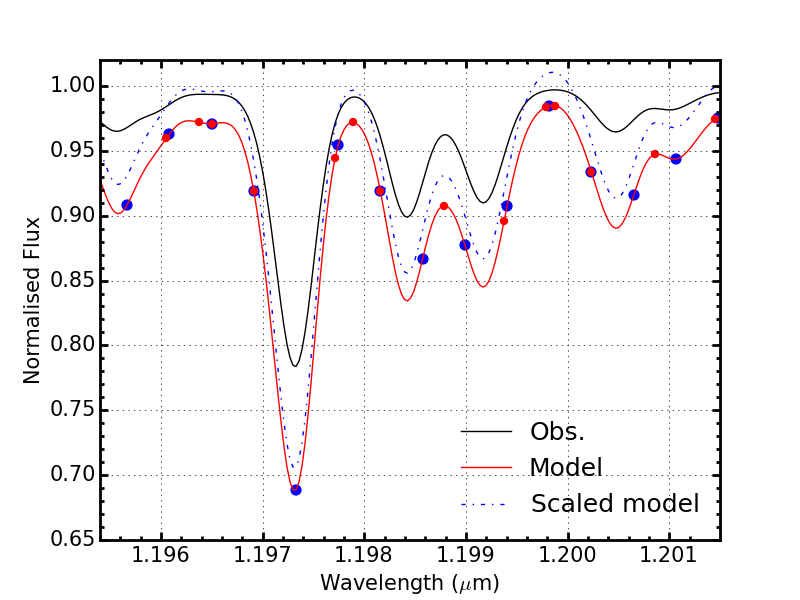
\includegraphics[width=0.65\textwidth]{JAnal/cftaction}
\caption[Example of continuum fitting]{
An example of the continuum fitting procedure using a model spectrum as an example observed spectrum (black solid line) and a separate model spectrum to match the level of the continuum.
The dashed blue spectrum denotes the model spectrum before any scaling has taken place.
The dot-dashed red spectrum denotes the model spectrum after the continuum fitting scaling has been applied.
The red and blue points indicate the edges of the slices made and maxima of these regions respectively.
For these models, the true continuum level is at 1.00.\label{fig:cftaction}
         }
\end{figure}

The remaining data points ($P_{cont}$) are used to derive an initial correction function
($cf_{init}$) by fitting a third-order polynomial to the ratio of the model to observed continuum points (red points in figure~\ref{fig:cw}), defined using the equation:
\begin{equation}
    cf_{init}~=~f\left(\frac{F_{mod}(P_{cont})}{F_{obs}(P_{cont})}\right),
    \label{eq:cf_init}
\end{equation}

\noindent where $F_{mod}$ and $F_{obs}$ are the flux in the model and observed spectrum respectively.
The final correction function ($cf_{fin}$), a refinement of $cf_{init}$,
is defined by removing any remaining outliers more than 3$\sigma$ from the mean of the initial correction function.
This method assumes that over the small wavelength range considered,
$cf_{init}$ does not vary significantly from the mean and as such, any significant deviation is considered originating from a spectral feature or noise.

The final correction function, $cf_{fin}$,
is used to define the amount of scaling required for the model.
Figure~\ref{fig:cft3pan} demonstrates how the continuum fitting process works in three panels by showing the observed spectrum (which in this case is an example model spectrum; black solid line) alongside the unscaled model spectrum in the top panel (red solid line), the continuum points -- derived from the model spectrum -- which are used to define $cf_{fin}$ are shown in the middle panel as well as the final correction function and the corrected model spectrum in the bottom panel.
In addition Figure~\ref{fig:cftaction} shows, on a smaller scale, how the continuum points and hence the the final correction function are defined.
It can be seen in from these two figures that the continuum placement of the example observed spectrum and that of the scaled model spectrum is well matched, even though the line strengths don't match well.

%  the continuum fitting process works using a model spectrum as the observed spectrum (black) and a second model spectrum
% (red solid line) which is scaled to match the continuum level of the observed
% (red dot-dashed).




% The green dashed line shows a third order polynomial fit to the ratio of the model spectrum to a simulated observed spectrum at only the red points ($~=~\frac{F_{mod}(cf_{init})}{F_{obs}(cf_{init})}$).

Alternative methods of continuum fitting are discussed in~\cite{2010MNRAS.407.1203D} and~\cite{2011A&A...527A..50E}.
These methods select pseudo-continuum pixels in the models based on ranking the model pixels and selecting a percentage of the pixels with the largest flux.
Providing the pixels from the model are selected in this manner and not those in the observations, this is a reliable method with which to derive the continuum level as demonstrated by~\cite{2015ApJ...806...21D}.

% section continuum_fitting (end)
\section{Best Fit Parameters} % (fold)
\label{sec:best_fit_parameters}

Best fit parameters are calculated using a maximum likelihood approach where the $\chi^{2}$-squared statistic is computed to compare the model and the observed spectra.
The $\chi^{2}$-squared statistic is calculated using the equation,

\begin{equation}
    \chi^{2}~=~\frac{1}{N_{pix}}\sum\limits_{i}{\frac{(O_{i} - M_{i})^{2}}{\sigma^{2}}},\label{eq:chisq}
\end{equation}

where $N_{pix}$ is the number of pixels used
% , $N_{lines}$ is the number of lines used
and $\sigma$ is determined by the S/N of the spectrum.
This statistic is calculated for each of the diagnostic lines where $N_{pix}$ is the total number of pixels within each line.
Table~\ref{tb:lines} details the diagnostic lines used in this analysis.
The amount of continuum included to compute the $\chi^{2}$-statistic is important to consider.
If this wavelength range is too small, the wings of the lines will be neglected,
which would discard vital information used to constrain the model parameters.
However, if too much of the pseudo-continuum is included, the parameters could be biased by noise features in the observations or by inaccuracies within the models.
% For example,
% ~\cite{2014PhDT.........G} identify several spectral features present in the observed spectra which are missing in the model spectra.

The regions which are used in the calculation of the $\chi^{2}$-statistic are highlighted red in
Figure~\ref{fig:lines}.
From a careful analysis of the individual spectra, the exact regions over which to compute the $\chi^{2}$-statistic are adjusted slightly depending upon the quality of the reduction and the appearance of reduction residuals near any lines of interest.

As a conservative estimate, for testing purposes, I use 10 regions corresponding to the cores of the individual lines.
In practise however, given that there are several lines which are sufficiently
close together that, at R~$\sim$~3000,
the lines are not clearly separated.
In these instances, the most appropriate course of action is often to define a region which encompassess all of the spectral features in question.
For example, the Fe\,\1$\lambda$1.188285 and the Ti\,\1$\lambda$1.189289
or the Fe\,\1$\lambda$1.197305 and Si\,\1$\lambda\lambda$1.198419, 1.199157 lines often are covered by one region to ensure that specific pixels are not counted multiple times.


\begin{figure}
 \centering
 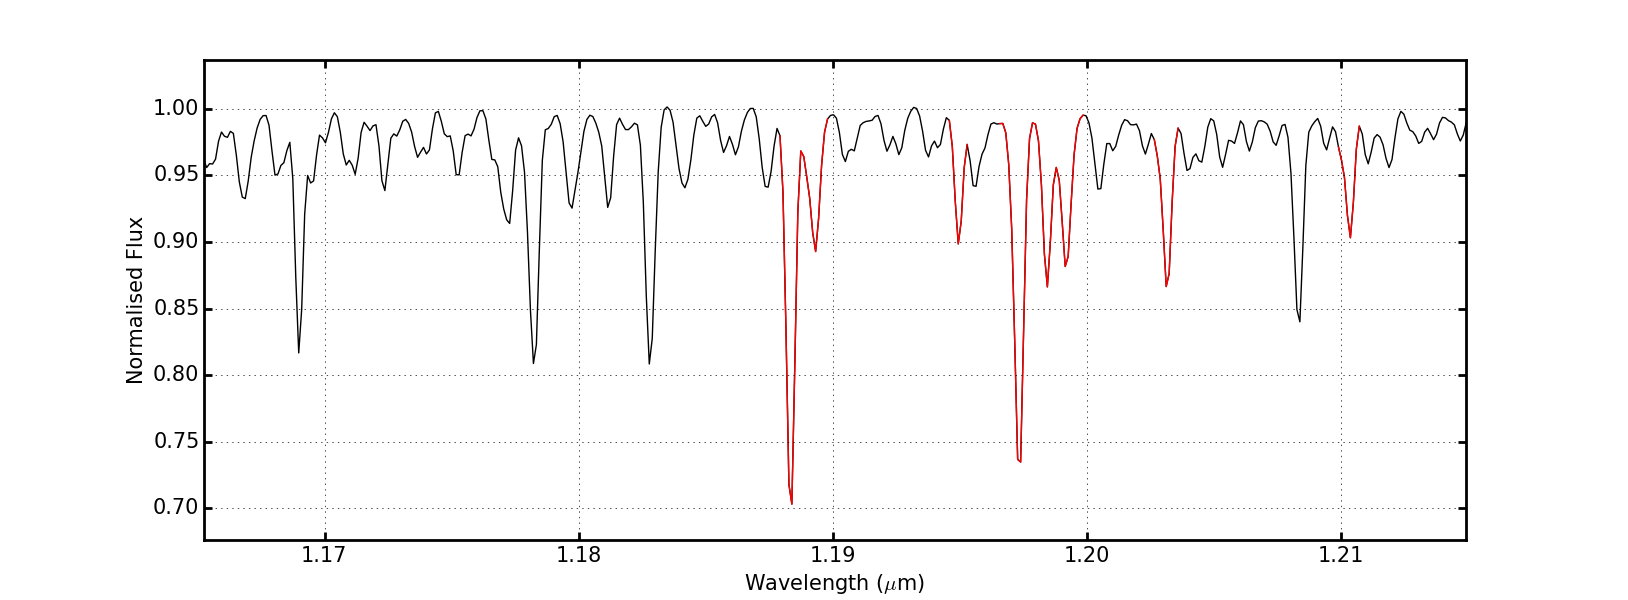
\includegraphics[width=\textwidth]{JAnal/Diag-lines}
 \caption[Diagnostic lines]{
An example of a model spectrum, degraded and resampled to that of a typical observed spectrum, where the regions used to compute the $\chi^{2}$ calculation are highlighted in red.
\label{fig:lines}
         }
\end{figure}

\begin{table}
\caption[Diagnostic lines]{Diagnostic lines used to estimate stellar parameters ordered by wavelength, by species.\label{tb:lines}}
\scriptsize
\begin{center}
\begin{tabular}{cc}
 \hline
 \hline
Species & Line Centre \\
 \hline
Fe\,I & 1.188285 \\
Fe\,I & 1.197305 \\
Si\,I & 1.198419 \\
Si\,I & 1.199157 \\
Si\,I & 1.203151 \\
Si\,I & 1.210353 \\
Ti\,I & 1.189289 \\
Ti\,I & 1.194954 \\
Mg\,I & 1.182819\\
Mg\,I & 1.208366\\
 \hline
\end{tabular}
\end{center}
\end{table}

The best-fit parameters are estimated based on a sampling of the posterior probability density function using {\sc emcee}
\cite{2013PASP..125..306F},
an implementation of the affine-invariant ensemble sampler for Markov chain Monte Carlo (MCMC) of~\cite{2010CAMCS.5..65G}.
The likelihood function used is
\begin{equation}
    p(D|\{[Z], \log g, \Teff, \xi\})~=~\exp(-\chi^{2}/2), \label{eq:like}
\end{equation}

\noindent where the data ($D$) consists of the observed spectra and $\chi^{2}$ is calculated as given by Equation~\ref{eq:chisq}.

The initial guess for each run of the MCMC sampler is based on some prior assumptions about the stars in question depending upon their location and distribution.
For example, in Chapter~\ref{ch:ngc2100}, where the RSGs in question are in a star cluster in the LMC, the initial guess is: [Z]~=~$-$0.3\,dex (i.e. LMC-like), $\log g$~=~0.0, \Teff~=~4000\,K and $\xi$=3.0.
The guess is varied assuming a Gaussian distribution with a mean value centred on the initial guess and the standard deviation is chosen such that, for each parameter, the guesses sample a majority of the available parameter space (defined by Table~\ref{tb:grid}).
In the absence of prior information on the metallicity parameter, as is the case with the other parameters, the mid-point of the grid is chosen.
% However, the best fit parameters and error estimation does not dependent upon the initial guesses.

To aid the {\it a priori} assumptions, if broad-band photometry is available for the objects in question
(which is nearly always the case given that the most common way to select RSGs is based on the optical or near-IR colours) this information is used to restrict the available range in parameter space.
To do this, the luminosity of the star is calculated using the bolometric corrections of~\citet{2013ApJ...767....3D} where the photometric band used is preferably the $K$-band to minimise the effects of interstellar extinction.
This is done by combining the two equations which were previously described as two of the fundamental equations for stellar atmospheres (equations~\ref{eq:grav} and~\ref{eq:Teff}) to arrive at the expression,

\begin{equation}
    \frac{g}{T^{4}_{\rm eff}}~\propto~\frac{M}{L}.
\end{equation}

By assuming sensible limits on the masses of RSGs, which are thought to be in the range 8~$\leq$~M/M$_{\odot}$~$\leq$~40, one can restrict the available range of the $\log g$ parameter by calculating an upper and lower estimates at every \Teff~grid space.
The models which have $\log g$ values outside of this allowed range are rejected as not physical.
This helps to minimise the number of $\chi$-squared calculations performed and also helps to break the $\log g$-[Z] degeneracy within the models.

The best fit parameters and errors are calculated by drawing at least 200\,000 independent samples from the probability density function (rejecting the first half of the results as ``burn-in'') and computing the
16$^{\rm th}$, 50$^{\rm th}$ and 84$^{\rm th}$ percentile as defined of these samples.
The quoted value for each parameter is then,

\begin{equation}
     x_{-\sigma_{low}}^{+\sigma_{high}}
\end{equation}
\noindent where $x$ is the 50$^{\rm th}$ percentile, $\sigma_{low}$ is the 50$^{\rm th}$ - 16$^{\rm th}$ percentiles and $\sigma_{high}$ is the 84$^{\rm th}$ - 50$^{\rm th}$ percentiles.
In practise, the upper and lower error bound are sufficiently consistent that the average of the two values is taken.
An exception to this is when a model parameter is on, or near the edge of available grid.
In this case, the largest of the upper and lower error bound is quoted as the error.


% Each best fit parameter is estimated based on a weighted average,
% where the weights are determined by the $\chi^{2}$ value of the model:

% \begin{equation}
%     w~=~exp(-\chi^{2}/2).
% \end{equation}

% The average is performed using the 100 models with the lowest $\chi^{2}$ value.
% \begin{itemize}
%     \item Why is 100 chosen?
%     \item Doesn't this bias models at the edge of the grid? (e.g. figure~\ref{fig:t2})
%     \item I need more on this in general!
% \end{itemize}

% Errors on the parameters are determined by defining
% $\Delta\chi^{2}~=~\chi^{2}_{min} + 3$.
% The standard deviation of the models parameters for all models which have a
% $\chi^{2}$ value within this range define the errors.
% For a purely Gaussin distribution the 1$\sigma$ deviation is $\Delta\chi^{2}~=~2.3$.
% However, assuming one of the diagnostic lines is only fit to within 2$\sigma$ while the rest being fit to within 1$\sigma$, we obtain $(n_{l}~-~1)~\times~1^{2}~+~1~\times~2^{2}~=~n_{l}~+~3$
% where $n_{l}$ is the number of lines used.

\section{Calibration} % (fold)
\label{sec:calibration}


To test the accuracy of this method of parameter estimation two main tests are devised which involve simulating observed data with fake RSG spectra of which the input parameters are known:

\begin{enumerate}
    \item Fake spectra at model resolution and high S/N and
    \item Fake spectra at typical observed resolution and S/N.
\end{enumerate}

In these tests the resolution of the models is degraded by using Gaussian filter, where the width of this function is determined by the output resolution (as described in Section~\ref{sec:continuum_fitting}).
Once the spectra have been degraded (if applicable), random Gaussian noise of with $\mu$~=0.0 and $\sigma$~=~1/(S/N) is added to each spectral channel.
The result of this process are idealised simulated observed data with known input parameters.
Idealised, in the sense that this method assumes no reduction residuals are present.
By comparing the parameters used to create the spectra (input) with the results of the analysis routine described above (ouput) one can assess the effectiveness and limitations of this analysis.

Figure~\ref{fig:t1} shows the results of test i using 18 fake RSG spectra, which show that in the simplest of tests this method is able to recover input parameters well.
The average difference between the input and output parameters for this test are
$\Delta\Teff$~=~$-$9.3\,$\pm$\,13.7,
$\Delta\log g$~=~$-$0.03\,$\pm$\,0.04,
$\Delta\xi$~=~$-$0.07\,$\pm$\,0.08 and
$\Delta[Z]$~=~$-$0.016\,$\pm$\,0.026
which are all consistent with there being no systematic offset between the input and output parameters.
The uncertainties quoted in Figure~\ref{fig:t1} are dominated by the uncertainties in the models.
Therefore, in order to prevent errors in the models causing unrealistic uncertainties,
the $\sigma$-values used in equation~\ref{eq:chisq} is never allowed to be smaller than $\sigma$~=~1/150.

\begin{figure}
 \centering
 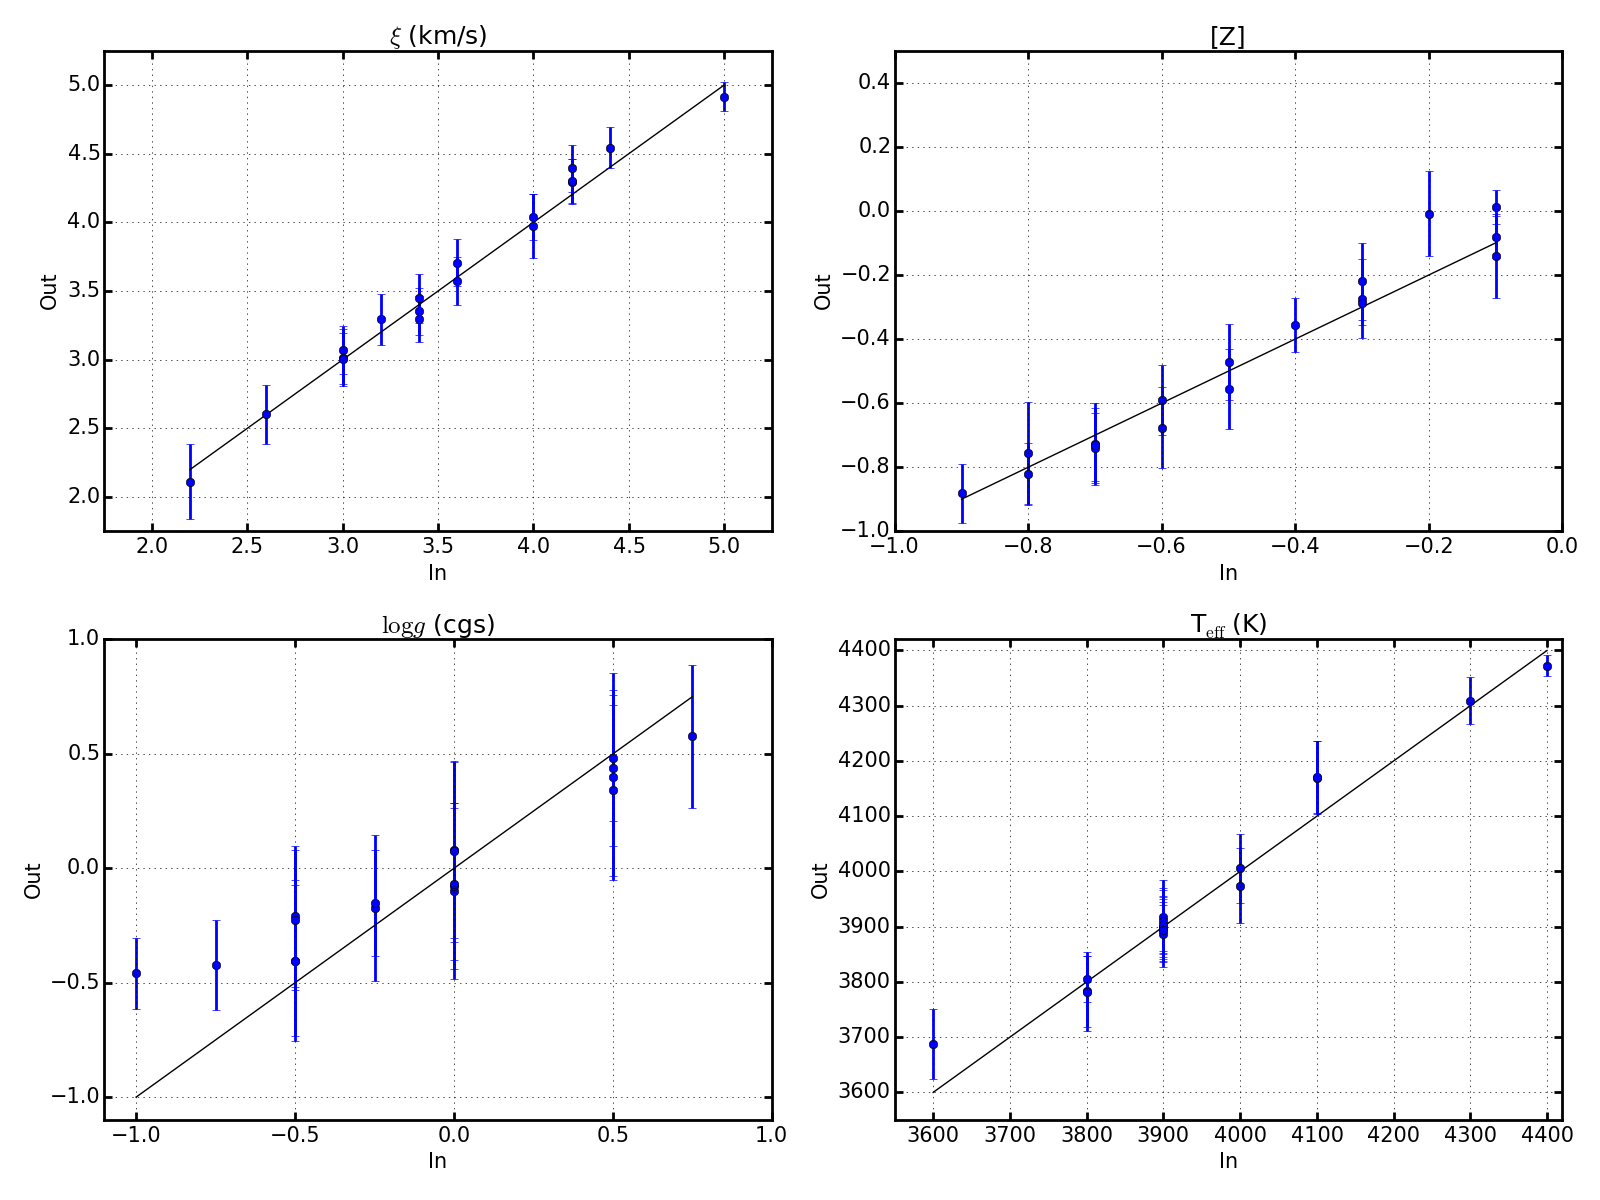
\includegraphics[width=0.80\textwidth]{JAnal/Fakespec-t1-v2}
 \caption[Analysis test i: Input against output parameters using fake RSG spectra at S/N~=~150 ($R$~=~10\,000)]{
 Analysis test i: Input Vs output parameters for fake spectra ($R$~10\,000) generated from models by including random Gaussian noise (S/N~=~150).
\label{fig:t1}
         }
\end{figure}


The results of test ii are displayed in Figure~\ref{fig:t2} where, again, the results compare well with the input parameters.
The average difference between the input and output parameters for this test are
$\Delta\Teff$~=~15.1\,$\pm$\,21.1,  % [INFO] DeltaTeff = 15.1+/-21.1
$\Delta\log g$~=~$-$0.10\,$\pm$\,0.10, % [INFO] Deltalog g = -0.10+/-0.10
$\Delta\xi$~=~0.03\,$\pm$\,0.07 and % [INFO] DeltaMicro Turb = 0.03+/-0.07
$\Delta[Z]$~=~$-$0.05\,$\pm$\,0.04     % [INFO] Delta[Z] = -0.05+/-0.04
which, again, are consistent with recovering the input parameters.
However, we note that there appears to be a small, low-significance, systematic offset in the $[Z]$ parameter.
This is an important offset to quantify, however, this offset is smaller than the typical error in this parameter, in addition, the significance of this offset is low.
Therefore, this offset is not accounted for in the final estimated [Z] parameter, however it is noted that it could explain a potential discrepancy between the results presented here and the results of an alternative implementation (see below).

To produce Figure~\ref{fig:snr} the model spectra are degraded to a resolution of $R$~=~3000 where the S/N~=~150 per pixel for each spectrum.
In addition, from an analysis of Figures~\ref{fig:t1} and~\ref{fig:t2} there appears to be a systematic shift to higher $\log g$ models towards the lower boundary of the model grid, however, this does not appear to be significant.
Figure~\ref{fig:t2} shows that in an ideal case, this analysis routine is able to accurately estimate stellar parameters at the typical resolution and S/N of KMOS spectra.

% # Test 2
% In [134]: run par-compare
% [INFO] Deltalog g = -0.10+/-0.10
% [INFO] DeltaMicro Turb = 0.03+/-0.07
% [INFO] Delta[Z] = -0.05+/-0.04

\begin{figure}
 \centering
 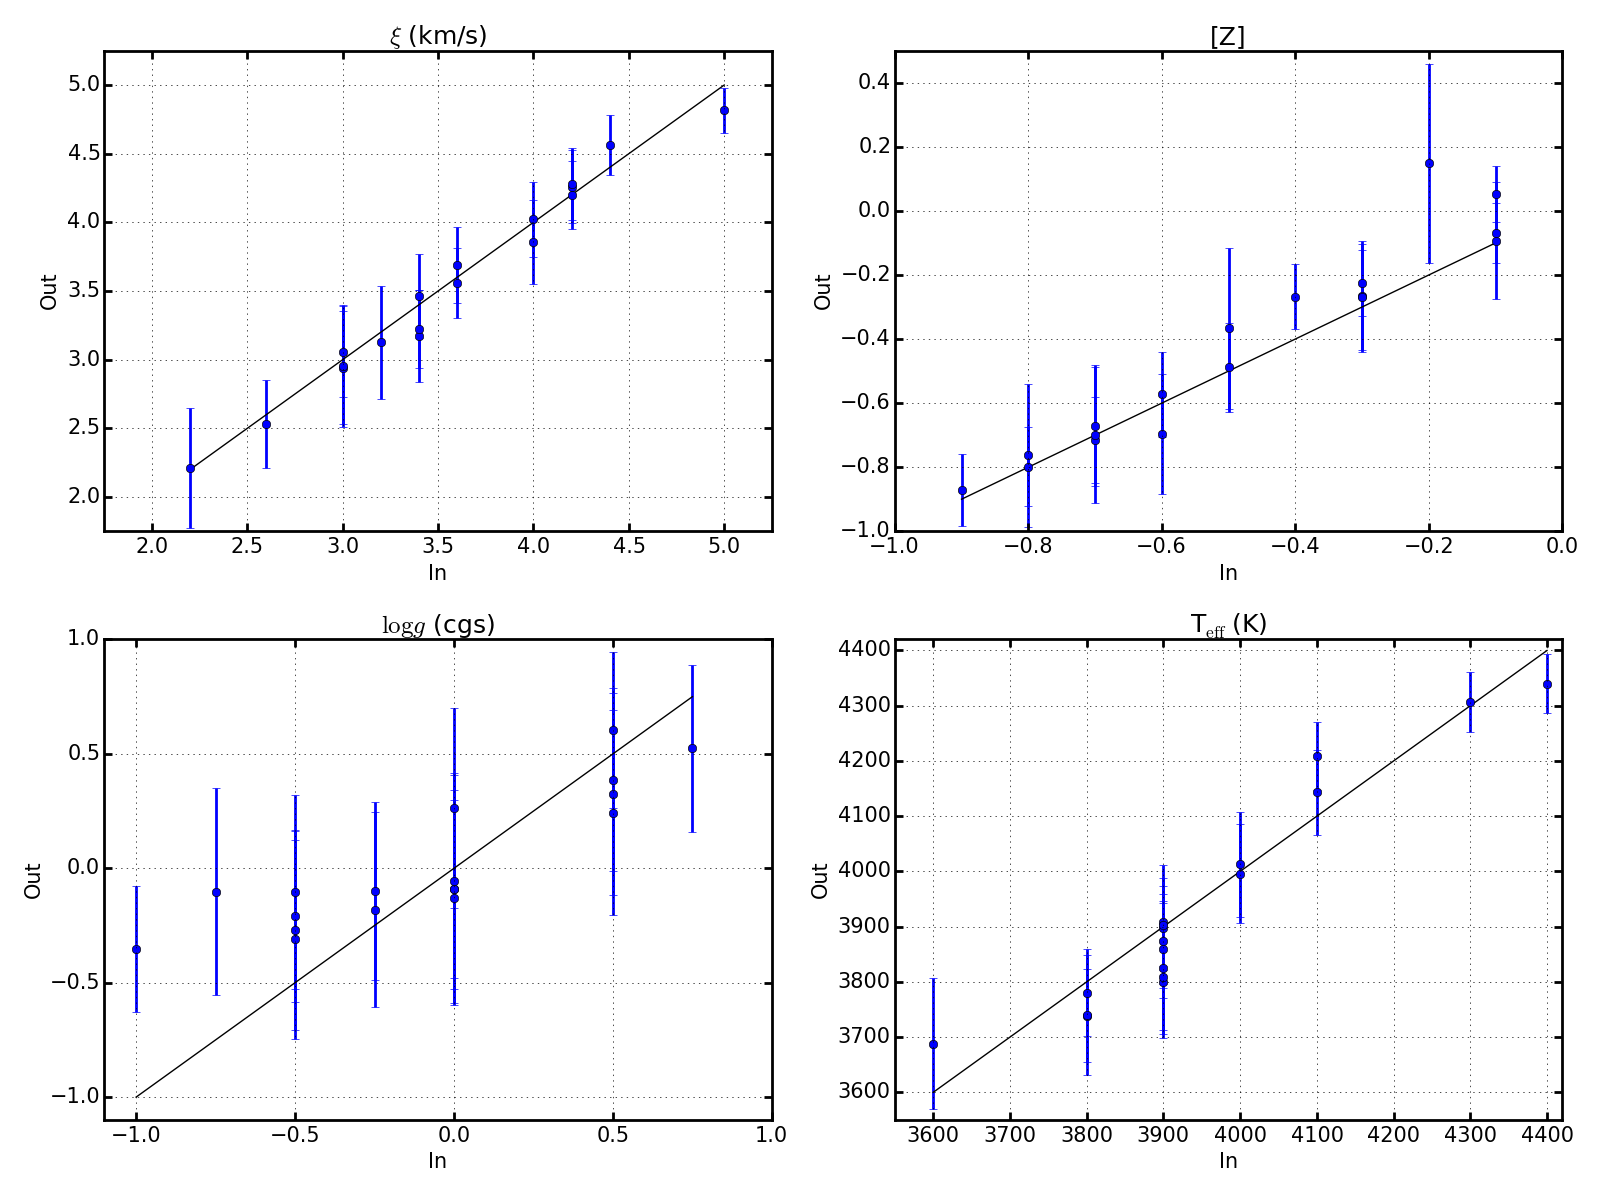
\includegraphics[width=0.80\textwidth]{JAnal/Fakespec-t2-v2}
 \caption[Analysis test ii: Input against output parameters using fake RSG spectra at S/N~=~150 ($R$~=~3000)]{
 Analysis test ii: Input Vs output parameters for fake spectra ($R$~3000) generated from models by including random Gaussian noise (S/N~=~150).
Gaussian noise is added after the spectra have been degraded.
This figure shows that the analysis technique presented is (in an ideal case) able to accurately estimate stellar parameters at the typical resolution and S/N of KMOS spectra.
\label{fig:t2}
         }
\end{figure}

In addition, it is useful to characterise how the fit parameters respond to the spectral resolution and S/N of the input spectra to assess the limits of this technique, particularly in the case of low spectral resolution and/or S/N.
Figure~\ref{fig:tres} shows input and output parameters for one model spectrum which is degraded to have different resolution values in the range 1000~$< R <$~10,000.
The green dashed line in each panel represents the respective input parameters for this model.
From this test we can see that the parameters appear stable to below $R$~=~3000, which is significant as the resolution of KMOS in the $YJ$-band is typically 3000~$< R <$~4000.
In addition, the uncertainties on the surface gravity parameter appears to be insensitive to the input resolution.
Note that the uncertainties on the parameters in Figure~\ref{fig:tres} are stable beyond R $\sim$ 5000 owing to the intrinsic uncertainties in the models.

\begin{figure}
 \centering
 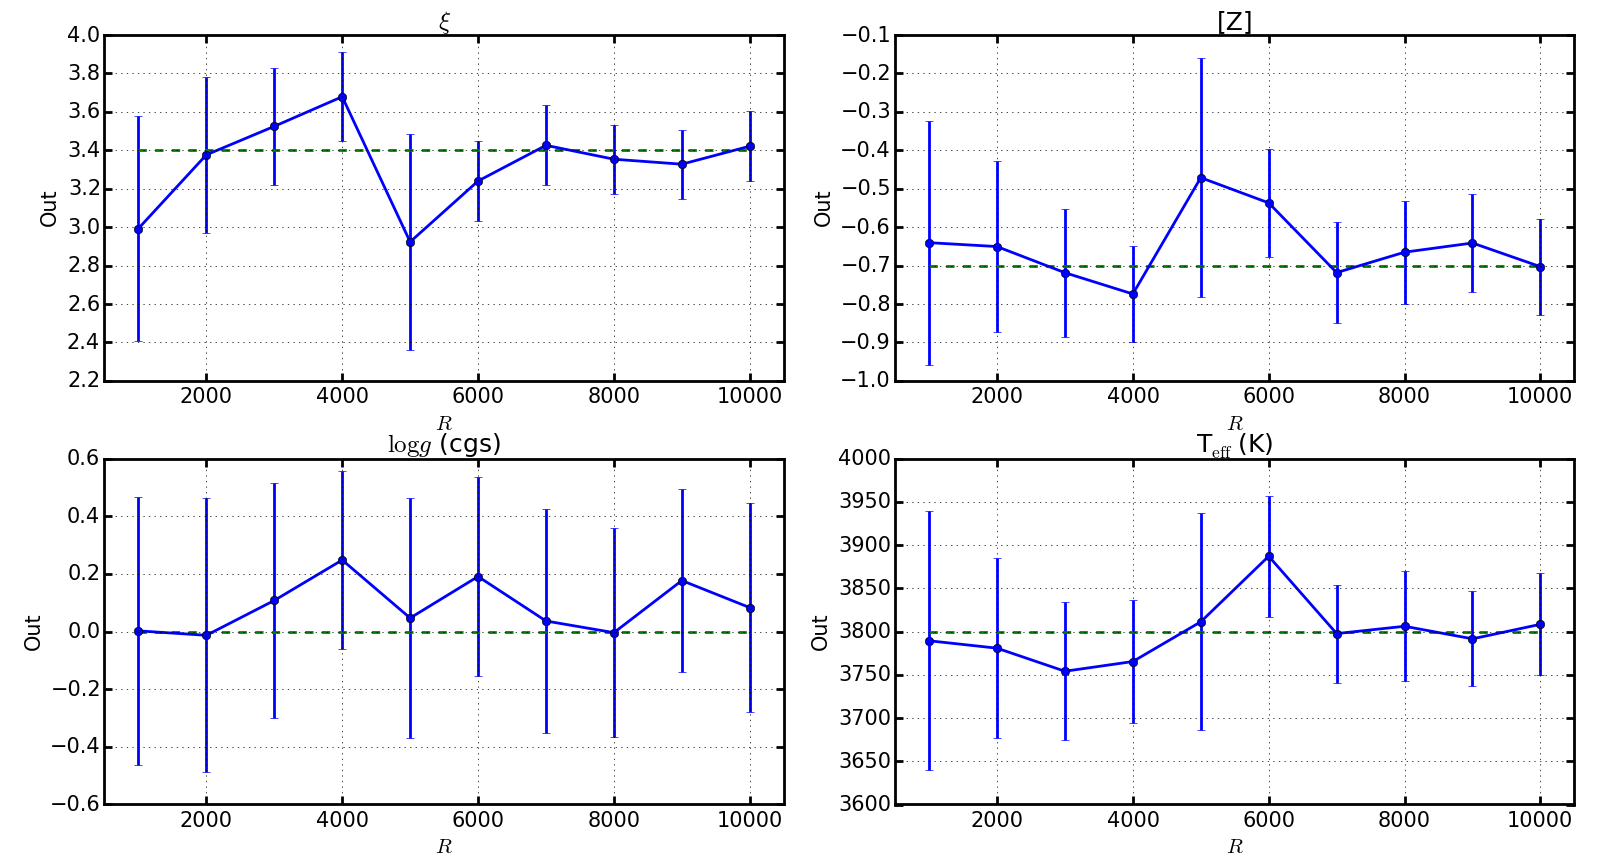
\includegraphics[width=0.80\textwidth]{JAnal/Fakespec-tres-v1}
 \caption[Analysis test resolution]{
Best fit parameters using a single fake RSG spectrum generated from a model spectrum by including random Gaussian noise (S/N~=~150) degraded to various resolution values in the range  to a resolution of $R$~=~3000 (and resampled onto the typical sampling for an KMOS spectrum) at varying S/N ratios in the range 50~$<$~S/N~$<$~150.
\label{fig:tres}
         }
\end{figure}

Figure~\ref{fig:snr} shows that best fit parameters for a single fake RSG spectrum degraded to a resolution of $R$~=~3000 (and resampled onto the typical sampling for an KMOS spectrum) at varying S/N ratios.
This figure shows that at the S/N ratios which is typical of KMOS observations of RSGs this technique is able to accurately estimate fit parameters.
We note however that with decreasing S/N regime of real spectra, the contribution of residuals from the reduction process becomes increasingly important.
Therefore for real observed data, we expect this analysis routine to break down at below S/N~=~100 at $R$~=~3000.

\begin{figure}
 \centering
 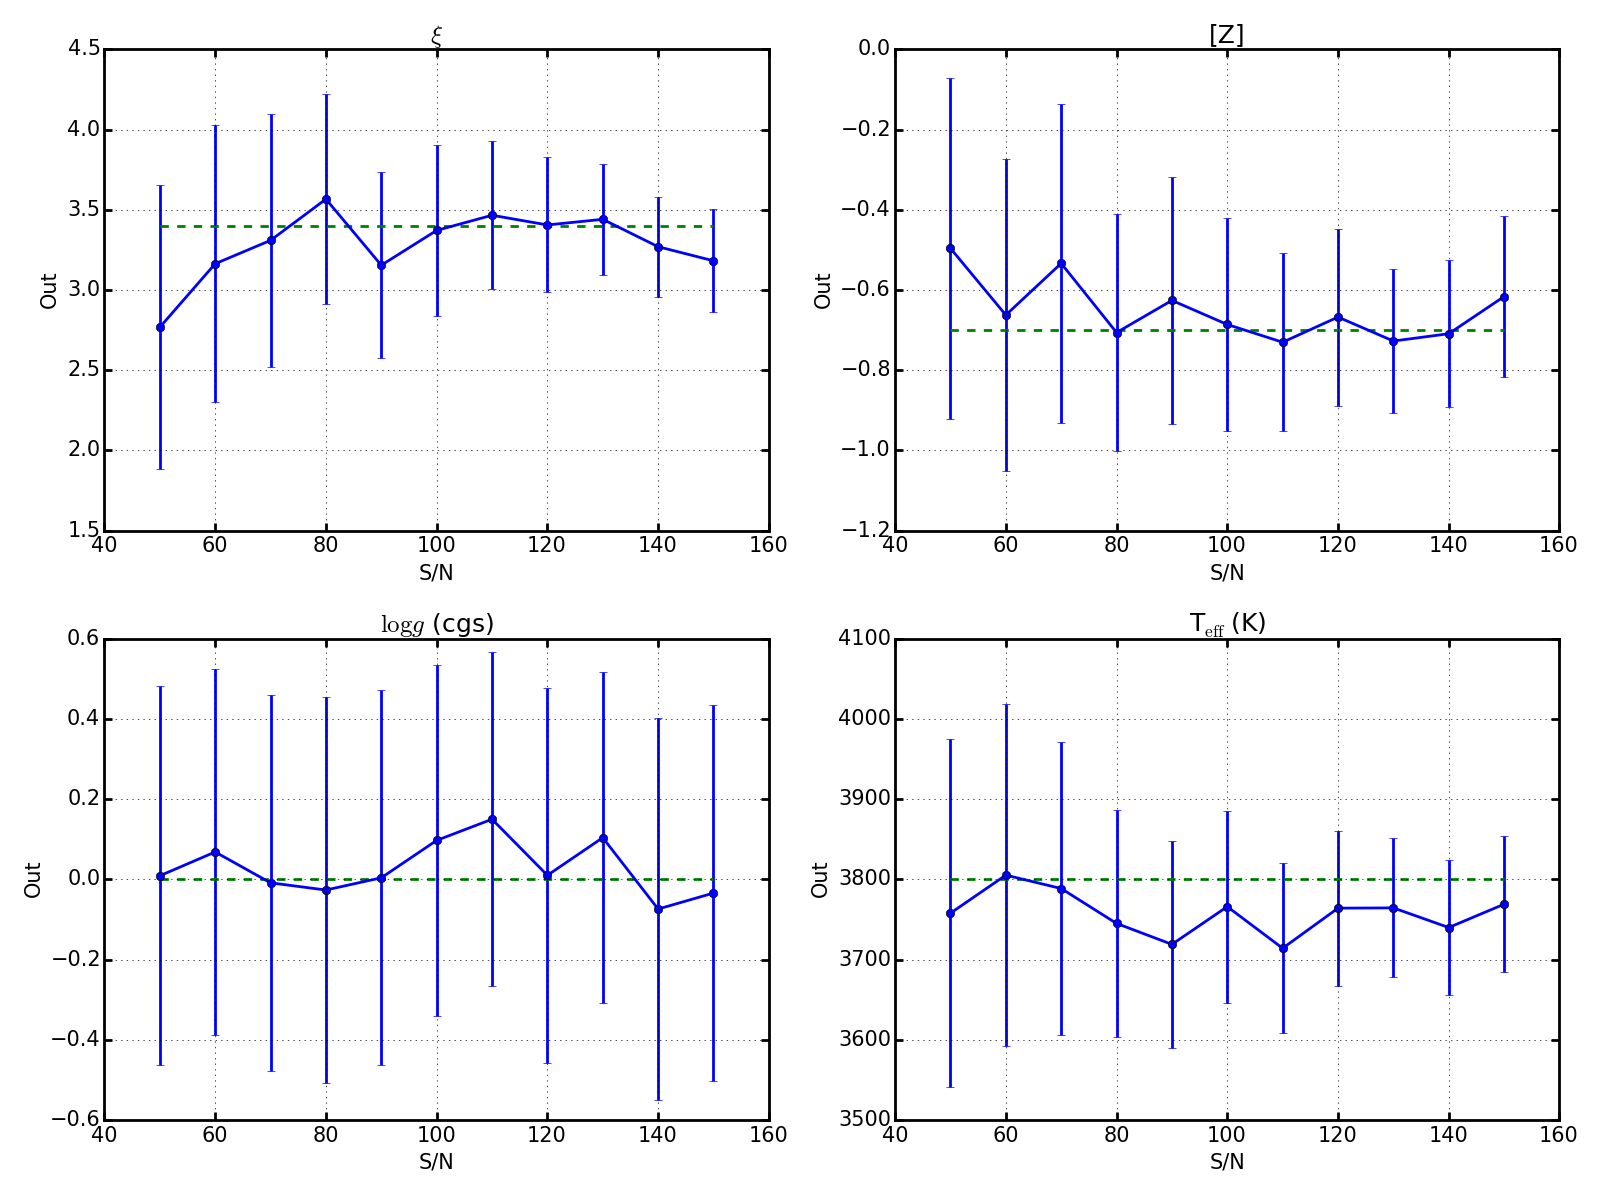
\includegraphics[width=0.80\textwidth]{JAnal/Fakespec-tsnr-v1}
 \caption[Analysis test S/N]{
Best fit parameters using a single fake spectrum degraded to a resolution of $R$~=~3000 (and resampled onto the typical sampling for an KMOS spectrum) at varying S/N ratios in the range 50~$<$~S/N~$<$~150.
\label{fig:snr}
         }
\end{figure}


As the analysis routine described above has been shown to be internally consistent, the natural next step is to compare the results of this technique with other similar techniques.
This helps to increase confidence in the accuracy and reliability in applying spectral fitting in the $J$-band to RSGs in general as well as providing a vital test on the effectiveness of the technique described in this thesis.

There are currently two other published analyses using medium resolution $J$-band spectra of RSGs to estimate stellar parameters,
those of~\cite[][DFK10]{2010MNRAS.407.1203D} and
\cite[][G14]{2014PhDT.........G}.
Both of these approaches use different assumptions to estimate the stellar parameters from a similar model grid.

The main differences between the two methods are that DFK10 uses the strengths of several diagnostic lines to compute the $\chi^{2}$ statistic,
while G14 uses a more extended region within the 1.165--1.215\,$\mu$m where several key diagnostic lines are present.

In the current analysis, the shape and strength of the diagnostic lines are used to calculate the $\chi^{2}$ statistic.
This is preferred to the two aforementioned techniques for the following reasons:

\begin{enumerate}
    \item The models used are not perfect representations of RSG spectra.
    The line list which builds these spectra are known to be incomplete and the effect of including these wavelength regions within the $\chi^{2}$ calculation could be to perturb the fit. G14 is very careful to exclude all known instances of missed lines within the models, however, this can not be assumed to be a complete consensus of omitted features.

    \item By using the full line profile of the diagnostic lines one can use the shape and strength of the lines to break degeneracies between model parameters.
\end{enumerate}

In addition, an updated line list is used in the current study.
This update includes the non-LTE effects on two strong magnesium lines within the region~\citep{2015ApJ...804..113B}.
In Chapter~\ref{ch:ngc6822} the difference between including and excluding these magnesium lines is explored.

To date there have been several published articles using the DFK10 analysis
~\citep{2010MNRAS.407.1203D,2015ApJ...806...21D,2015ApJ...803...14P}.
This technique has been updated and tested rigorously on VLT-XSHOOTER spectra of RSGs in the Magellanic clouds in
~\cite{2015ApJ...806...21D} and in~\citet[][which Chapter~\ref{ch:ngc6822} is based upon]{2015ApJ...803...14P} this was applied to KMOS spectra in NGC\,6822.

Here the best fit parameters from~\cite{2015ApJ...803...14P} are compared with the results of the presented technique.
In addition, results presented in~\citep{2016arXiv160202702P} and Chapter~\ref{ch:ngc55} are also compared (Davies 2016, Private communication).

Figures~\ref{fig:n6822DFK} and~\ref{fig:n2100DFK} show the comparison of the output parameters of the stars in the NGC\,2100 and NGC\,6822 samples for the two analysis routines.
These figures show that, in general, the agreement between the two routines is acceptable for all stellar parameters.
The mean of each of the parameters and average offsets are calculated in Table~\ref{tb:DFK10} and are shown to agree within the errors.

% \textbf{Comment on individual cases?}

Therefore I conclude that the presented analysis routine is able to accurately measure stellar parameters of RSGs given a set of synthetic spectra extracted from model atmospheres.
Compared to DFK10 results from the NGC\,2100 and NGC\,6822 data sets the stellar parameters generally agree well, however, the average offset for the surface gravity parameter appears to be larger than can be accounted for by the uncertainties on the measurements.
This could be the result of an underestimate of the uncertainties in the current implementation as, in general, the uncertainties reported in this study on this parameter are smaller than those estimated using the DFK method.

\begin{figure}
 \centering
 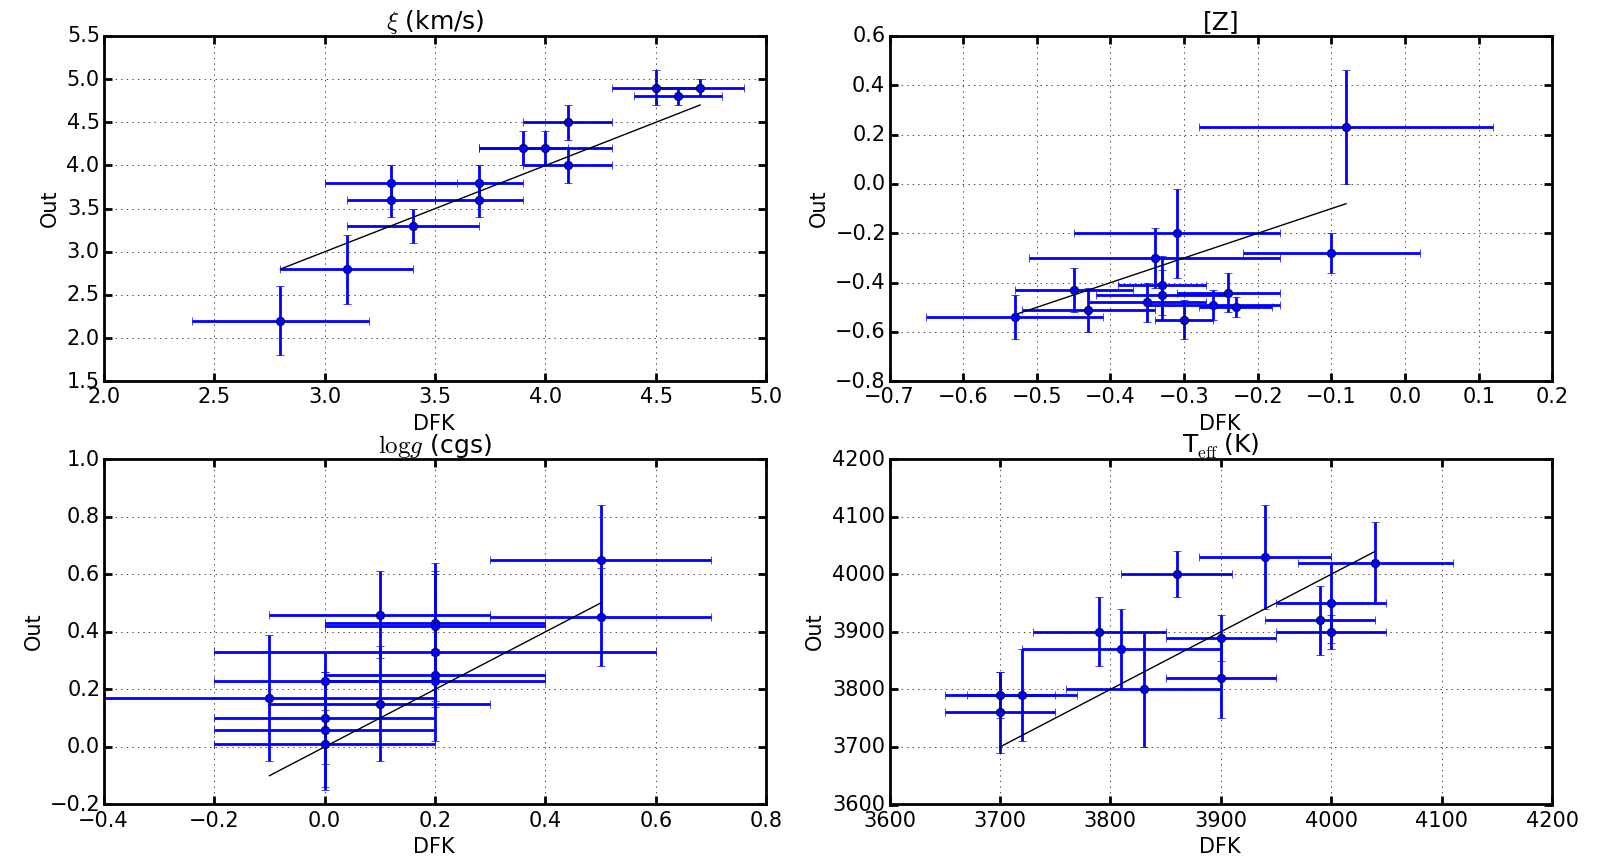
\includegraphics[width=0.80\textwidth]{JAnal/NGC2100-par-compare}
 \caption[NGC\,2100 DFK10 best fit parameter comparison]{
A comparison between the best-fit parameters derived for 14 RSGs in NGC\,2100.
DFK10 results are those published in~\cite{2016arXiv160202702P}.
\label{fig:n2100DFK}
         }
\end{figure}

\begin{figure}
 \centering
 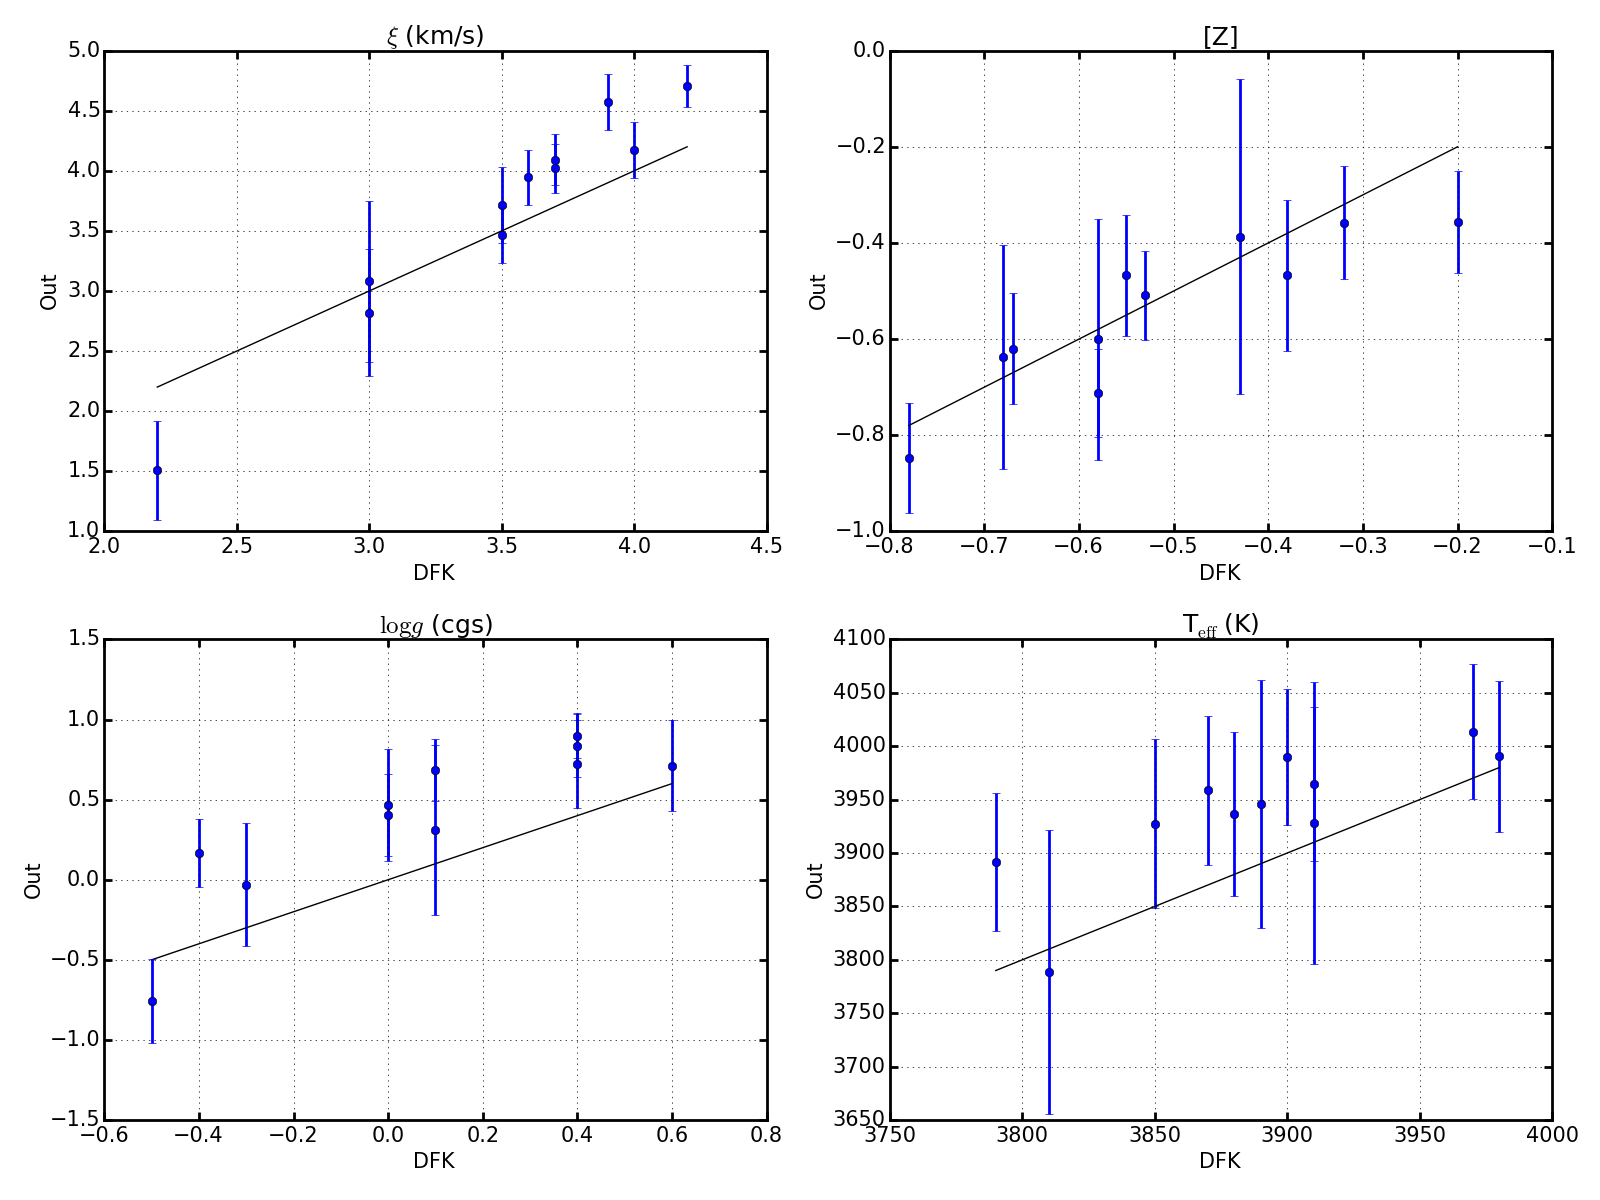
\includegraphics[width=0.80\textwidth]{JAnal/NGC6822-par-compare}
 \caption[NGC\,6822 DFK10 best-fit parameter comparison]{
A comparison between the best fit parameters derived for 11 RSGs in NGC\,6822.
DFK10 results are those published in~\cite{2015ApJ...803...14P}.
\label{fig:n6822DFK}
         }
\end{figure}

\begin{table}
\caption[Parameter comparisons DFK10]{Average parameters for RSGs in NGC\,2100 and NGC\,6822 using the DFK10 parameter estimation technique and the technique described here\label{tb:DFK10}}
\scriptsize
\begin{center}
\begin{tabular}{c ccc c ccc}
 \hline
 \hline
Parameter & \multicolumn{3}{c}{NGC\,2100} &  & \multicolumn{3}{c}{NGC\,6822}\\
  \cline{2-4}  \cline{6-8}
          & DFK10 & Current & $\Delta \overline{X}$  & & DFK10 & Current & $\Delta \overline{X}$\\
 \hline
\Teff           & 3870\,$\pm$\,110       &3900\,$\pm$\,85\o\a     & $-$19\,$\pm$\,25    & & 3890\,$\pm$\,55      & 3940\,$\pm$\,60\o\a        & $-$52\,$\pm$\,40\\
$\log g$        & \o0.15\,$\pm$\,0.17    &0.25\,$\pm$\,0.15       & $-$0.13\,$\pm$\,0.08& & \o\a0.07\,$\pm$\,0.34    & 0.40\,$\pm$\,0.46      & $-$0.33\,$\pm$\,0.17\\
$\xi$           & \o3.8\,$\pm$\,0.6      &4.0\,$\pm$\,0.6         & $-$0.1\,$\pm$\,0.1  & & \o\a3.5\,$\pm$\,0.5      & 3.6\,$\pm$\,0.9        & $-$0.2\,$\pm$\,0.2\\
\lbrack Z\rbrack& $-$0.31\,$\pm$\,0.12\p &$-$0.43\,$\pm$\,0.10\o\p& $-$0.08\,$\pm$\,0.04& & \v$-$0.52\,$\pm$\,0.16 & $-$0.54\,$\pm$\,0.15\o\p & \pp0.02\,$\pm$\,0.08\\
 \hline
\end{tabular}
\end{center}
\end{table}

% The second implementation of the $J$-band analysis technique using $J$-band spectra of RSGs was that presented and rigorously tested in~\cite{2014PhDT.........G}.
% This implementation was set up to be complementary to that of DFK10 and was tested on high resolution spectra of RSGs in the Perseus OB-1 cluster.
% In addition to this, this analysis was applied to KMOS spectra of 27 RSGs of NGC\,300
% \citep{2015ApJ...805..182G}.

% Stellar parameters have been for all spectra in NGC\,300 using the presented analysis.
% In figure~\ref{fig:n300G14} I compare the results derived using the analysis presented here with those published in~\citep{2015ApJ...805..182G}.
% Table~\ref{tb:G14} shows a comparison between the the mean and standard deviation of the four parameters.
% The metallicity gradient is also derived for these observations and is found to compare ...

% As part of the analysis G14 also fit for the resolution of the observations as a free parameter.
% The resolution for each spectrum is compared to that of the values quoted in the KMOS arc-lamp calibrations.
% \textbf{I'm expecting to see that these numbers are very similar}


% \begin{figure}
%  \centering
%  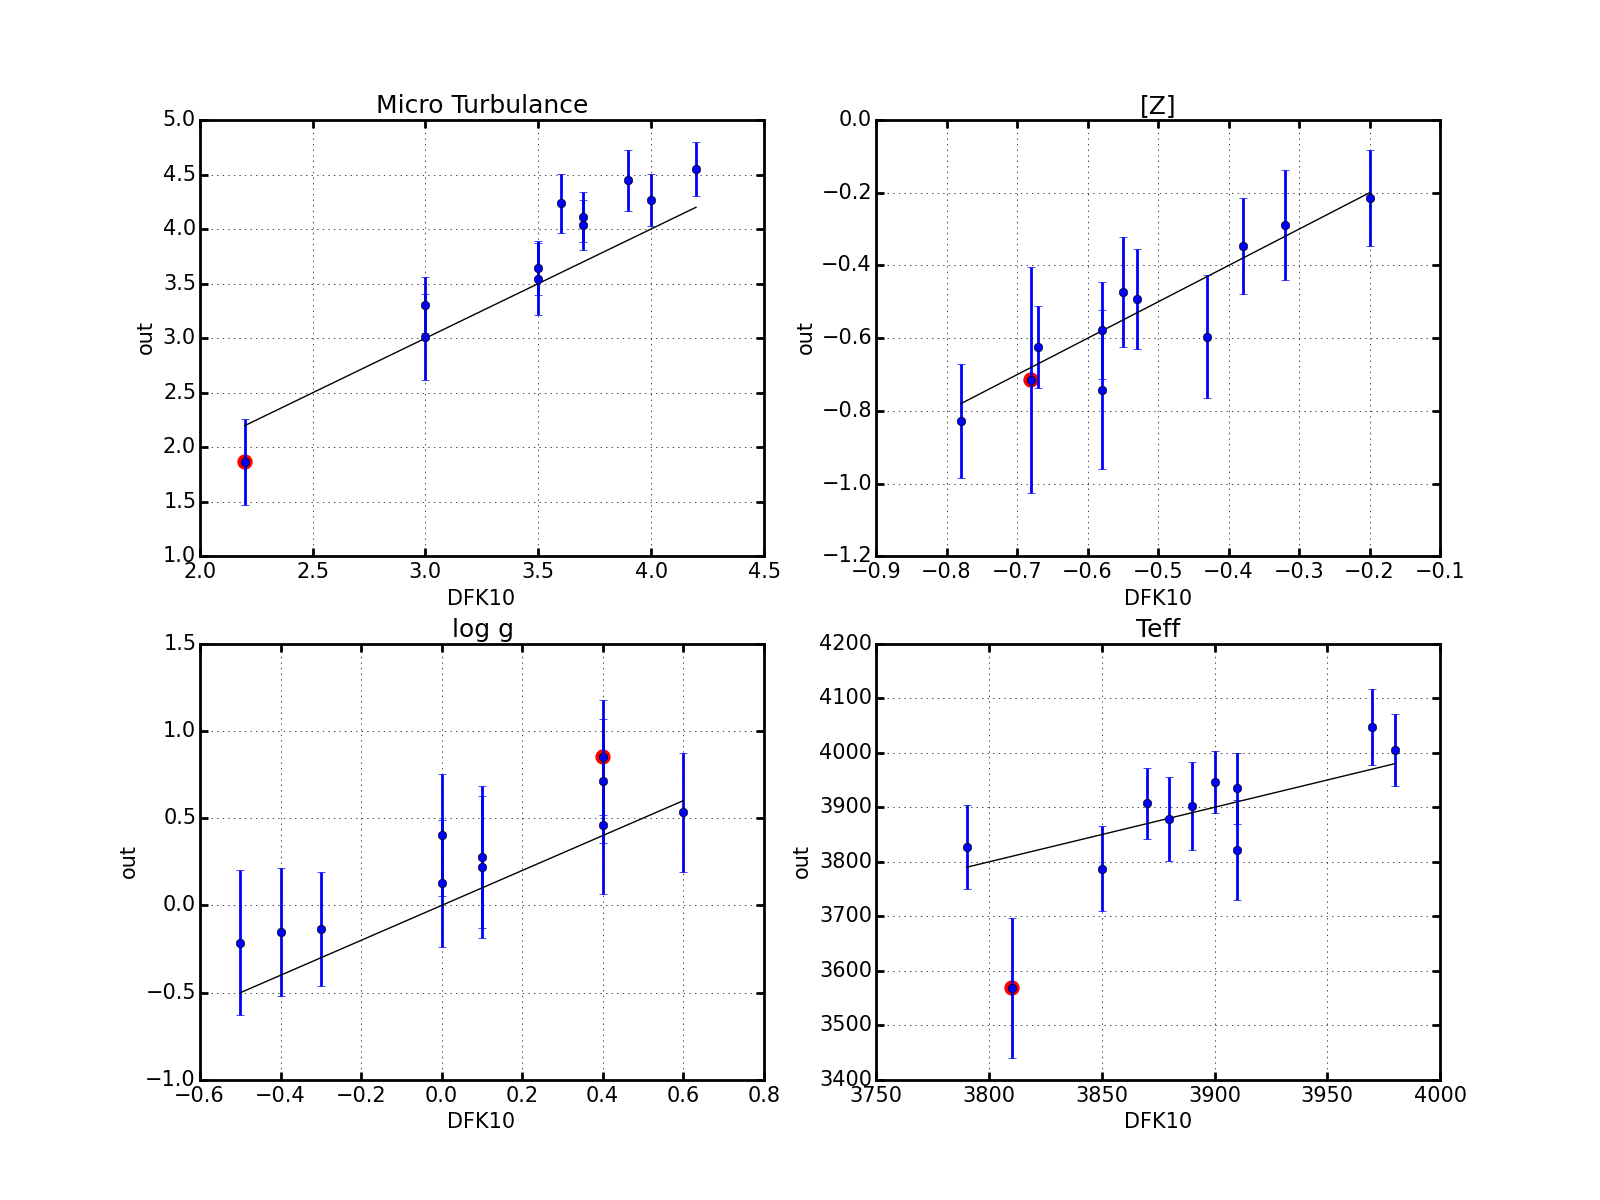
\includegraphics[width=0.65\textwidth]{JAnal/compare-DFK10}
%  \caption[NGC\,300 G14]{
% A comparison between the parameters derived for 27 RSGs in NGC\,300.
% DFK10 results are those published in~\cite{2015ApJ...805..182G}.
% \textbf{Placeholder}\label{fig:n300G14}
%          }
% \end{figure}

% \begin{table}
% \caption[Parameter comparisons G14]{Average parameters for 27 RSGs in NGC\,300 using the G14 implementation and the implementation described here
% \textbf{Place holder!}\label{tb:G14}}
% \scriptsize
% \begin{center}
% \begin{tabular}{ccc}
%  \hline
%  \hline
% Parameter & G14 Average & Patrick Average \\
%  \hline
% [Z]       & $-0.52~\pm~0.16$ &  \\
% \Teff & $3887~\pm~55$ &  \\
% $log\,g$  & $0.1~\pm~0.3$ &  \\
% $\xi$     & $3.9~\pm~0.5$ &  \\
%  \hline
% \end{tabular}
% \end{center}
% \end{table}

% section calibration (end)

\section{Conclusions} % (fold)
\label{sec:conclusions}

In this chapter I present an analysis routine which uses a grid of spectra extracted from stellar model atmospheres to estimate stellar parameters using medium resolution $J$-band spectroscopy of RSGs.

Initially, I give a description of stellar atmospheres focusing on their key assumptions and limitations.
Having described the background, I then detail the model stellar atmospheres used in the present study and describe the corrections made to include the non-LTE effects of the strongest diagnostic lines.
I then describe the steps taken to estimate best fit stellar parameters where the $\chi$-squared statistic is used to generate the posterior probability density function which is then sampled using an affine-invariant ensemble sampler.

The analysis is then tested using various fake spectra generated from the model grid (at different resolution and S/N) and show that this routine is internally consistent.
Finally, this technique is then thoroughly compared with that of DFK10 on all of the data sets used within this thesis and is shown to compare well with no significant systematic offsets.

% subsection conclusions (end)
% \bibliography{../journals,../books}
